\chapter{Arhitektura i dizajn sustava}

		
	\noindent Ključne komponente za ostvarenje našeg sustava: 
	   \begin{packed_item}
	        \item Web poslužitelj 
	        \item Web aplikacija 
	        \item Baza podataka
	    \end{packed_item}
	    
	
	%ARHITEKTURA SUSTAVA
	\begin{figure}[H]
		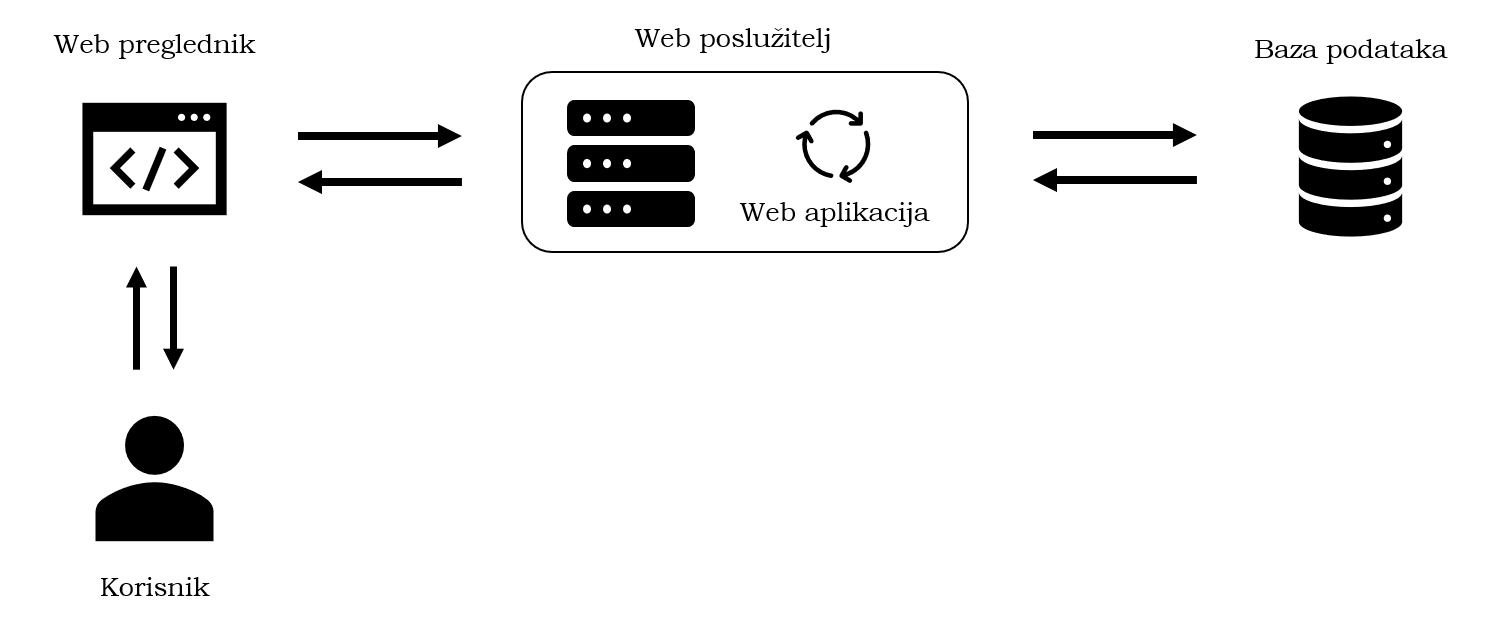
\includegraphics[scale=0.48]{slike/system-architecture.PNG} 
		\centering
		\caption{Arhitektura sustava}
		\label{fig:arhitektura}
	\end{figure}
		
	\noindent Komunikacija krajnjeg korisnika s našim sustavom započinje u web pregledniku pristupom iz javne mreže preko odgovarajuće poveznice. Konceptualnu shemu navedenog sustava moguće je pratiti na slici \ref{fig:arhitektura}.	 \par
	
	\medskip
	
	\noindent \underbar{Web preglednik} (engl. \textit{web browser}) program je koji korisniku omogućuje pronalaženje i pregled podataka na Internetu u obliku web stranica. Pruža grafičko sučelje i prikaz multimedijalnih sadržaja dohvaćenih s poslužitelja te prati korisničke akcije nad sučeljem kako bi generirao odgovarajuće zahtjeve i delegirao posao prema dijelu sustava koji ih obrađuje. Korišteni tip zahtjeva jest HTTP (engl. \textit{Hyper Text Transfer Protocol}). \par
	
	\medskip
	
	\noindent \underbar{Web poslužitelj} (engl. \textit{web server}) prima zahtjeve web preglednika. U našoj implementaciji pristupa mu se pomoću REST (engl. \textit{Representational State Transfer}) usluga koje koriste JSON format. Pokreće komunikaciju s web aplikacijom i prosljeđuje joj korisničke zahtjeve.  \par
	
	\medskip
	
	\noindent \underbar{Web aplikacija} (engl. \textit{web app}) je ključni dio sustava koji obrađuje korisničke zahtjeve. Obrada uključuje određenu komunikaciju s bazom podataka poput dohvata, uređivanja ili brisanja. Nakon što se odgovarajuće procesuira zahtjev, šalje se odgovor poslužitelju koji se ultimativno prikazuje korisniku u web pregledniku. \par
	
	
	
	\bigskip    
	
	
	
	\noindent Naš se produkt konceptualno temelji na troslojnoj arhitekturi kojom se najčešće koriste poslovne aplikacije i sastoji se od sljedećih slojeva:
	 \begin{packed_enum}
	        \item \textbf{Prezentacijski sloj} - korisničko sučelje aplikacije koje korisniku predstavlja značajke i podatke aplikacije
	        \item \textbf{Servisni sloj} - sadrži poslovnu logiku koja pokreće osnovne funkcionalnosti aplikacije poput donošenja odluka, izračuna, procjena i obrade podataka koji prolaze između druga dva sloja
	        \item \textbf{Podatkovni sloj} - odgovoran za interakciju s bazama podataka radi spremanja i vraćanja podataka aplikacije
	    \end{packed_enum}
	
	\bigskip
	
	\noindent Specifičnije, korišteni Spring razvojni okvir koristi se i MVC arhitekturom (eng. \textit{Model-View-Controller}). To podrazumijeva sljedeću podjelu uloga vidljivoj i na slici \ref{fig:mvc}.
	 \begin{packed_item}
	        \item \textbf{Model} - dohvat i manipulacija podatcima
	        \item \textbf{Pogled} - prezentacija dostavljenih podataka
	        \item \textbf{Nadglednik}  - prima zahtjeve te upravlja s pogledom i modelom
	 \end{packed_item}
	 
	%MVC ARHITEKTURA
	\begin{figure}[H]
		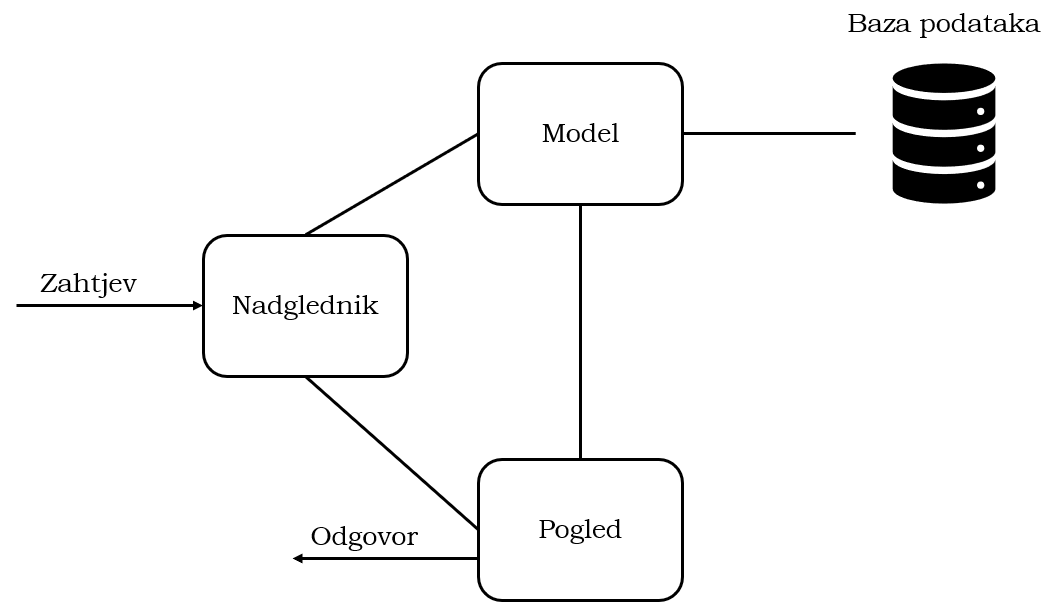
\includegraphics[scale=0.55]{slike/mvc-architecture.PNG} 
		\centering
		\caption{MVC arhitektura}
		\label{fig:mvc}
	\end{figure}
	
	\newpage

	
	 U prošlosti se linearnost troslojnog modela smatrala poželjnom, no razvojem web tehnologija "trokutasti" MVC model dobio je na popularnosti pa danas mnogi sustavi koriste hibridnu formu navedenih arhitekturnih oblika pa tako i Spring razvojni okvir. 
	
	%HIBRIDNA ARHITEKTURA
	\begin{figure}[H]
		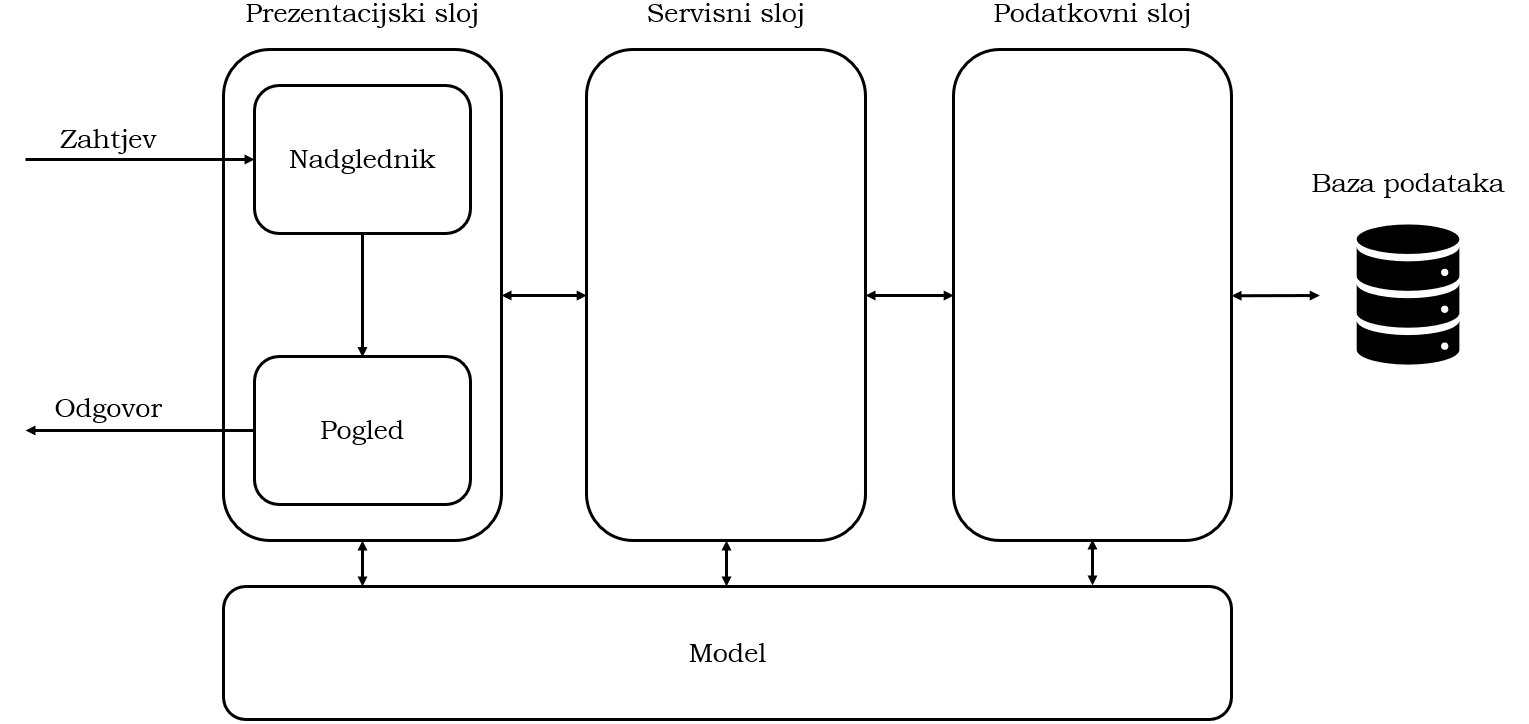
\includegraphics[scale=0.47]{slike/hybrid-architecture.PNG} 
		\centering
		\caption{Konceptualno hibridna arhitektura Spring razvojnog okvira}
		\label{fig:hibridna}
	\end{figure}
		

				
		\section{Baza podataka}
			
		
			Kako bi olakšali modeliranje stvarnog svijeta korištena je relacijska baza podataka. Modelirana je relacijama, odnosno tablicama koje imaju svoje ime i atribute. Tablice su različito povezane preko zajedničkih atributa. Baza podataka služi za brzu i jednostavnu pohranu podataka, izmjenu, ažuriranje te dohvat podataka za daljnju obradu. Ova aplikacija koristi bazu podataka sa sljedećim entitetima:
			
			\begin{packed_item}
				
				\item  RegisteredUser
				\item  RegisteredUserLogin
				\item  Association
				\item  AssociationLogin
				\item  Dog
				\item  WalkJournal
				\item  AssociationLocation
				\item  DogAvailability
				\item  RankingList
				\item  OtherReservations
				
			\end{packed_item} 
		
			\subsection{Opis tablica}
			
					\noindent \textbf{Walker} Entitet sadrži sve bitne informacije o registriranom korisniku aplikacije. Njegovi atributi su: ID korisnika, ime i prezime, elektronička pošta i broj mobitela korisnika, javnost podataka i obrisan (atribut koji postaje true ako korisnik obriše svoj račun). Entitet RegisteredUser je u \textit{Many-to-One} vezi s entitetom RankingList preko jedinstvenog identifikatora korisnika i u \textit{One-to-Many} vezi s entitetom WalkJournal preko jedinstvenog identifikatora korisnika.
				
				\begin{longtabu} to \textwidth {|X[8, l]|X[6, l]|X[18, l]|}
					
					\hline \multicolumn{3}{|c|}{\textbf{Walker}}	 \\[3pt] \hline
					\endfirsthead
					
					\hline \multicolumn{3}{|c|}{\textbf{Walker}}	 \\[3pt] \hline
					\endhead
					
					\hline 
					\endlastfoot
					
					\cellcolor{LightGreen}UserID & BIGINT	&  	Jedinstveni identifikator korisnika 	\\ \hline 
					FirstName & VARCHAR	& Ime korisnika 		\\ \hline
					LastName & VARCHAR & Prezime korisnika \\ \hline
					Email & VARCHAR & Elektronička pošta korisnika \\ \hline
					PhoneNumber & VARCHAR & Broj mobitela korisnika \\ \hline
					Public & BOOLEAN & Javnost podataka korisnika \\ \hline
					Deleted & BOOLEAN & Račun obrisan \\ \hline
					
					
				\end{longtabu}
				
					\noindent \textbf{WalkerLogin} Entitet sadrži podatke za prijavu korisnika na aplikaciju. Njegovi atributi su: identifikator korisnika, korisničko ime i lozinka. Entitet WalkerLogin je u \textit{One-to-One} vezi s entitetom Walker preko jedinstvenog identifikatora korisnika.
				
				\begin{longtabu} to \textwidth {|X[8, l]|X[6, l]|X[18, l]|}
					
					\hline \multicolumn{3}{|c|}{\textbf{WalkerLogin}}	 \\[3pt] \hline
					\endfirsthead
					
					\hline \multicolumn{3}{|c|}{\textbf{WalkerLogin}}	 \\[3pt] \hline
					\endhead
					
					\hline 
					\endlastfoot
					
					\cellcolor{LightGreen}UserID & BIGINT	&  	Jedinstveni identifikator korisnika 	\\ \hline 
					UserName & VARCHAR	& Korisničko ime za prijavu 		\\ \hline
					Password & VARCHAR & Lozinka za prijavu \\ \hline 
					
					
				\end{longtabu}
				
				\noindent \textbf{Association} Entitet sadrži sve bitne informacije o registriranoj udruzi za pse. Njegovi atributi su: ID, OIB i naziv udruge, ime i prezime vlasnika udruge, elektroničku pošta, web-stranica udruge, opis, web-adresa logo-a udruge, telefonski broj za kontaktiranje udruge i obrisan (atribut koji postaje true ako udruga obriše svoj račun). Entitet Association je u \textit{One-to-One} vezi s entitetom AssociationLocation preko jedinstvenog identifikatora udruge i u \textit{One-to-Many} vezi s entitetom Dog preko jedinstvenog identifikatora udruge.
				
				\begin{longtabu} to \textwidth {|X[8, l]|X[6, l]|X[18, l]|}
					
					\hline \multicolumn{3}{|c|}{\textbf{Association}}	 \\[3pt] \hline
					\endfirsthead
					
					\hline \multicolumn{3}{|c|}{\textbf{Association}}	 \\[3pt] \hline
					\endhead
					
					\hline 
					\endlastfoot
					
					\cellcolor{LightGreen}AssociationID & BIGINT	&  	Jedinstveni identifikator udruge 	\\ \hline
					AssociationOIB	& VARCHAR & OIB udruge	\\ \hline 
					Name & VARCHAR & Naziv udruge \\ \hline
					FirstName & VARCHAR	& Ime vlasnika udruge 		\\ \hline
					LastName & VARCHAR & Prezime vlasnika udruge \\ \hline 
					Email & VARCHAR & Elektronička pošta udruge \\ \hline
					WebAddress & VARCHAR & Web-stranica udruge  \\ \hline
					Description & VARCHAR & Opis udruge \\ \hline
					PictureURL & VARCHAR & Logo udruge \\ \hline
					PhoneNumber & VARCHAR & Kontaktni broj udruge \\ \hline
					Deleted & BOOLEAN & Račun obrisan \\ \hline
					
					
				\end{longtabu}
				
				\noindent \textbf{AssociationLogin} Entitet sadrži podatke za prijavu udruge na aplikaciju. Njegovi atributi su: identifikator udruge, korisničko ime i lozinka. Entitet AssociationLogin je u \textit{One-to-One} vezi s entitetom Association preko jedinstvenog identifikatora udruge.
				
				\begin{longtabu} to \textwidth {|X[8, l]|X[6, l]|X[18, l]|}
					
					\hline \multicolumn{3}{|c|}{\textbf{AssociationLogin}}	 \\[3pt] \hline
					\endfirsthead
					
					\hline \multicolumn{3}{|c|}{\textbf{AssociationLogin}}	 \\[3pt] \hline
					\endhead
					
					\hline 
					\endlastfoot
					
					\cellcolor{LightGreen}AssociationID & BIGINT	&  	Jedinstveni identifikator udruge 	\\ \hline 
					UserName & VARCHAR	& Korisničko ime za prijavu 		\\ \hline
					Password & VARCHAR & Lozinka za prijavu \\ \hline 
					
					
				\end{longtabu}
				
				\noindent \textbf{Dog} Entitet sadrži informacije o psu koji je registriran u udruzi. Atributi tog entiteta su: ID psa, ID udruge u kojoj je registriran, ime psa, pasmina, web-adresa slike psa, preferirani način šetnje, opis psa i obrisan (atribut koji postaje true ako udruga obriše psa). Entitet Dog je u \textit{One-to-One} vezi s entitetom DogAvailabilty preko jedinstvenog identifikatora psa, u \textit{Many-to-One} vezi s entitetom Association preko jedinstvenog identifikatora udruge te u \textit{Many-to-One} vezi s entitetom WalkJournal preko jedinstvenog identifikatora psa.
				
				\begin{longtabu} to \textwidth {|X[8, l]|X[6, l]|X[18, l]|}
					
					\hline \multicolumn{3}{|c|}{\textbf{Dog}}	 \\[3pt] \hline
					\endfirsthead
					
					\hline \multicolumn{3}{|c|}{\textbf{Dog}}	 \\[3pt] \hline
					\endhead
					
					\hline 
					\endlastfoot
					
					\cellcolor{LightGreen}DogID & BIGINT	&  Jedinstveni identifikator psa	\\ \hline
					\cellcolor{LightBlue}AssociationID	& BIGINT &  ID udruge u kojoj se nalazi pas	\\ \hline 
					Name & VARCHAR & Ime psa \\ \hline
					Breed & VARCHAR	& Pasmina \\ \hline
					PictureURL & VARCHAR & Web-adresa slike psa \\ \hline
					PreferredWalkStyle & VARCHAR & Preferirani način šetnje psa(individualna ili grupna šetnja) \\ \hline
					Description & VARCHAR & Opis psa \\ \hline
					Deleted & BOOLEAN & Pas obrisan \\ \hline
					
				\end{longtabu}
				
				\noindent \textbf{Reservation} Ovaj entitet sadrži podatke o šetnjama. Atributi su: ID rezervacije šetnje, ID korisnika koji je šetao psa/e, datum šetnje, datum šetnje, vrijeme početka i kraja šetnje, način šetnje te informaciju o tome je li šetnja otkazana ili ne. Entitet WalkJournal je u \textit{Many-to-One} vezi s entitetom Walker preko jedinstvenog identifikatora korisnika, u \textit{One-to-Many} vezi s entitetom Dog preko jedinstvenog identifikatora psa te u \textit{Many-to-One} vezi s entitetom ReservationDogList preko jedinstvenog identifikatora rezervacije šetnje.
				
				\begin{longtabu} to \textwidth {|X[8, l]|X[6, l]|X[18, l]|}
					
					\hline \multicolumn{3}{|c|}{\textbf{Reservation}}	 \\[3pt] \hline
					\endfirsthead
					
					\hline \multicolumn{3}{|c|}{\textbf{Reservation}}	 \\[3pt] \hline
					\endhead
					
					\hline 
					\endlastfoot
					
					\cellcolor{LightGreen}ReservationID & BIGINT	&  Jedinstveni identifikator rezervacije šetnje	\\ \hline
					\cellcolor{LightBlue}UserID	& BIGINT & Jedinstveni identifikator korisnika koji je šetač	\\ \hline 
					date & DATE	& Datum zakazane šetnje \\ \hline
					StartTime & TIME	& Vrijeme početka šetnje \\ \hline
					ReturnTime & TIME	& Vrijeme povratka iz šetnje \\ \hline
					WalkStyle & VARCHAR & Način šetnje(individualna/grupna) \\ \hline
					Cancelled & BOOLEAN & Je li šetnja otkazana \\ \hline
					
				\end{longtabu}
				
				\noindent \textbf{AssociationLocation} Ovaj entitet sadrži podatke o lokacijama na kojima se nalazi udruga. Atributi ovog entiteta su: ID udruge, grad, ulica i kućni broj adrese udruge. Entitet AssociationLocation je u \textit{One-to-One} vezi s entitetom Association preko jedinstvenog identifikatora udruge.
				
				\begin{longtabu} to \textwidth {|X[8, l]|X[6, l]|X[18, l]|}
					
					\hline \multicolumn{3}{|c|}{\textbf{AssociationLocation}}	 \\[3pt] \hline
					\endfirsthead
					
					\hline \multicolumn{3}{|c|}{\textbf{AssociationLocation}}	 \\[3pt] \hline
					\endhead
					
					\hline 
					\endlastfoot
					
					\cellcolor{LightBlue}AssociationID & BIGINT	&  Jedinstveni identifikator udruge	\\ \hline
					City & VARCHAR & Grad \\ \hline
					Street & VARCHAR & Ulica \\ \hline
					HouseNumber & VARCHAR & Kućni broj \\ \hline
					
				\end{longtabu}
				
				\noindent \textbf{DogAvailability} Entitet sadrži podatke o vremenu kada je pas slobodan za šetnju. Atributi tog entiteta su: ID psa, datum, vrijeme od i vrijeme do kada se može rezervirati šetnja. Entitet DogAvailability je u \textit{One-to-One} vezi s entitetom Dog preko jedinstvenog identifikatora psa.
				
				\begin{longtabu} to \textwidth {|X[8, l]|X[6, l]|X[18, l]|}
					
					\hline \multicolumn{3}{|c|}{\textbf{DogAvailability}}	 \\[3pt] \hline
					\endfirsthead
					
					\hline \multicolumn{3}{|c|}{\textbf{DogAvailability}}	 \\[3pt] \hline
					\endhead
					
					\hline 
					\endlastfoot
					
					\cellcolor{LightBlue}DogID & BIGINT	&  Jedinstveni identifikator psa	\\ \hline
					StartDate & DATE & Datum od kada se može rezervirati šetnja \\ \hline
					EndDate & DATE & Datum do kada se može rezervirati šetnja \\ \hline
					StartTime & TIME & Vrijeme od kada se može rezervirati šetnja \\ \hline
					EndTime & TIME & Vrijeme do kada se može rezervirati šetnja \\ \hline
					Deleted & BOOLEAN & Oznacava je li dostupnost obrisana \\ \hline
					
				\end{longtabu}
			
				\noindent \textbf{ReservationDogList} Ovaj slabi entitet služi kao popis pasa koji su bili u šetnji u jednoj rezervaciji. Ključ ovog entiteta je jedinstveni identifikator rezervacije i identifikator psa. Entitet ReservationDogList je u \textit{One-to-Many} vezi s entitetom WalkJournal preko jedinstvenog identifikatora rezervacije.
				
				\begin{longtabu} to \textwidth {|X[8, l]|X[6, l]|X[18, l]|}
					
					\hline \multicolumn{3}{|c|}{\textbf{ReservationDogList}}	 \\[3pt] \hline
					\endfirsthead
					
					\hline \multicolumn{3}{|c|}{\textbf{ReservationDogList}}	 \\[3pt] \hline
					\endhead
					
					\hline 
					\endlastfoot
					
					\cellcolor{LightBlue}ReservationID & BIGINT	&  Jedinstveni identifikator rezervacije	\\ \hline
					\cellcolor{LightBlue}DogID & BIGINT	&  Jedinstveni identifikator psa	\\ \hline
					
				\end{longtabu}
			
			
			\subsection{Dijagram baze podataka}
				
				\begin{figure}[H]
    			    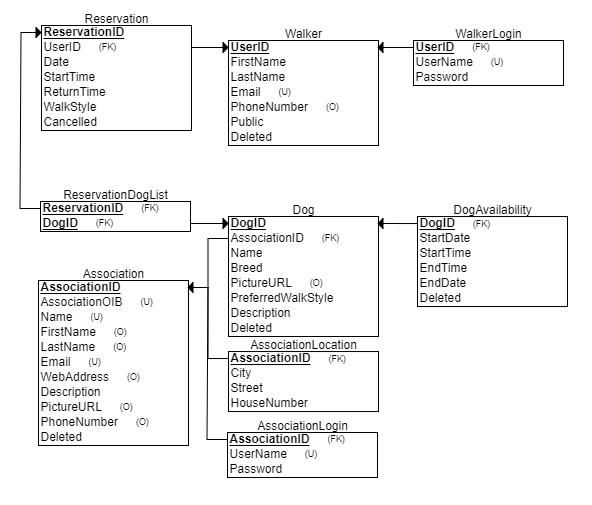
\includegraphics[scale=1.2]{dijagrami/database-scheme.png}
    			    \centering
    			    \caption{Dijagram baze podataka}
    			    \label{fig:shema}
		        \end{figure}
			
			\eject
			
			
		\section{Dijagram razreda}
		
			Dijagrami razreda omogućavaju pojednostavljen pogled i lakše razumijevanje komponenti arhitekture objektno orijentiranog sustava. Razredi sustava izrađenih u Springu prate norme razvojnog okvira. U našem sustavu zato imamo četiri glavna paketa i odgovarajuće potpakete. Njihov sadržaj moguće je vidjeti na sljedećim slikama:
			
			\begin{packed_item}
				\item[$\bullet$]  \textbf{domain} - Slika \ref{fig:classdiagram-domain}
				\item[$\bullet$]  \textbf{repository} - Slike \ref{fig:classdiagram-repository} i \ref{fig:classdiagram-repository-jpa}
				\item[$\bullet$]  \textbf{service} - Slika \ref{fig:classdiagram-service}
				    \begin{itemize}
				            \item[$\bullet$] \textbf{impl} - Slika \ref{fig:classdiagram-service-impl}
				    \end{itemize}
				\item[$\bullet$]  \textbf{rest} - Slika \ref{fig:classdiagram-rest}
				    \begin{itemize}
				        \item[$\bullet$] \textbf{dto} - Slika \ref{fig:classdiagram-rest-dto}
				    \end{itemize}
			\end{packed_item} 
			
			
			\begin{figure}[H]
    			    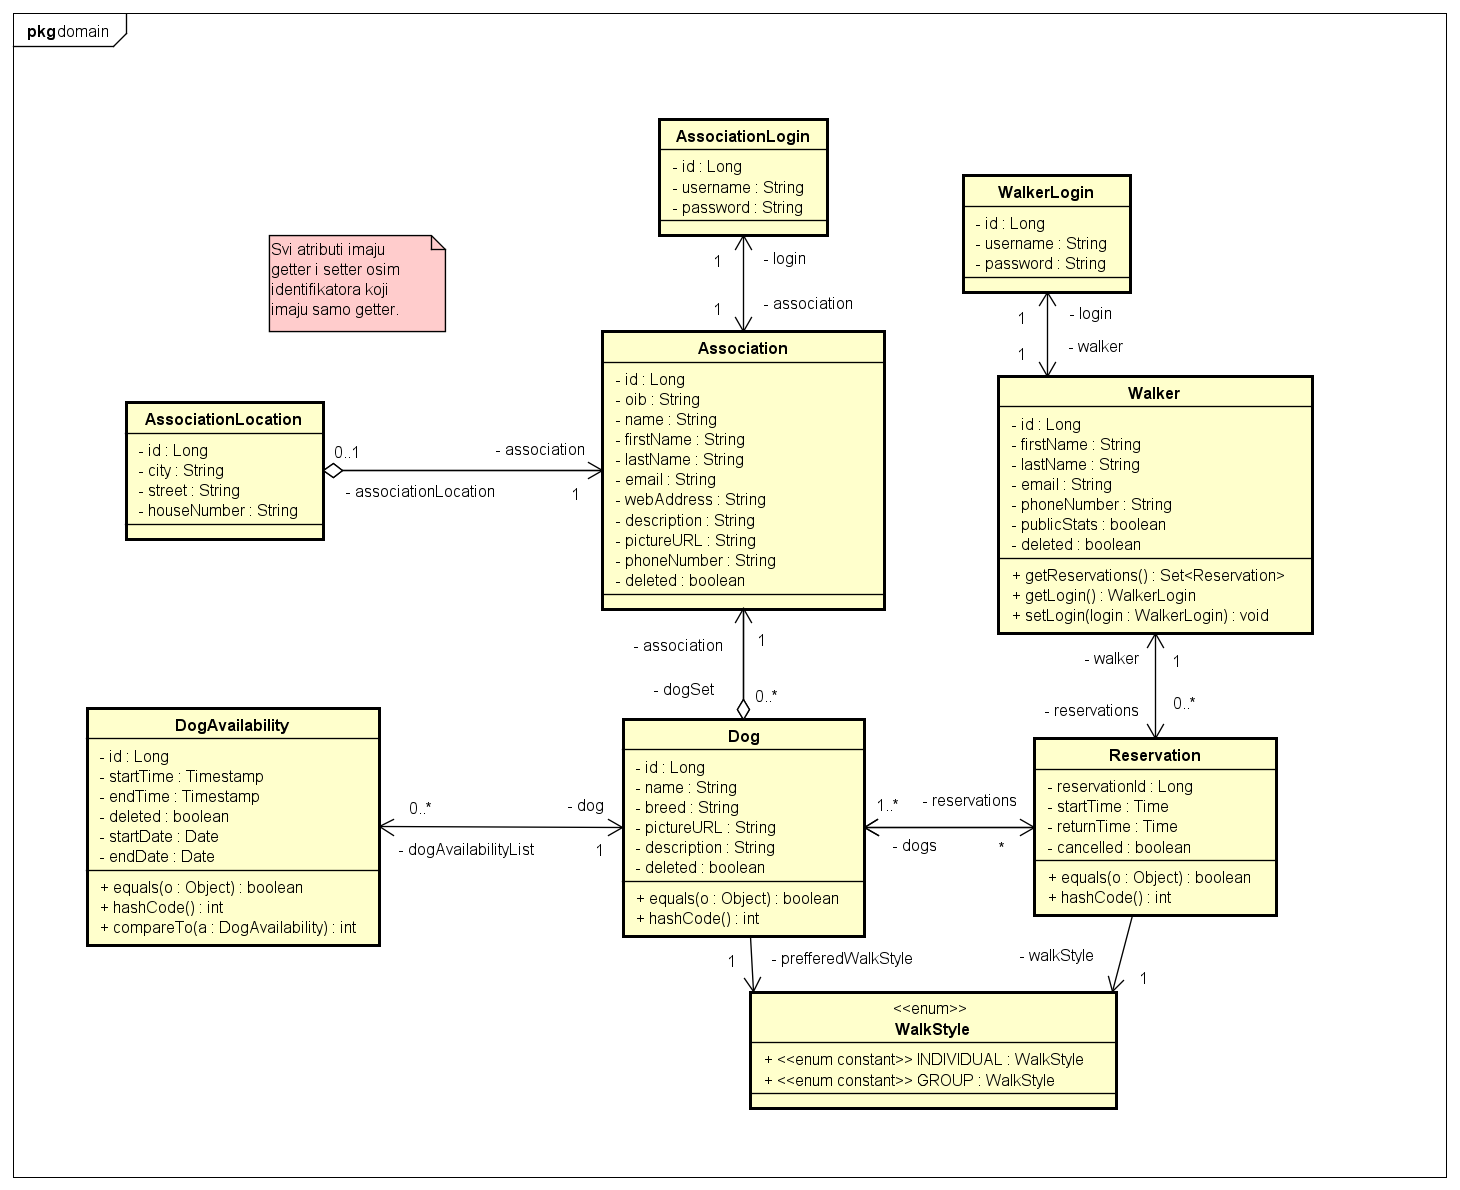
\includegraphics[scale=0.38]{dijagrami/classdiagram-domain.png}
    			    \centering
    			    \caption{Dijagram domenskih razreda}
    			    \label{fig:classdiagram-domain}
		    \end{figure}
		    
		    \noindent Na dijagramima je moguće vidjeti da kod prati načela troslojne arhitekture navedena na početku poglavlja. Klase paketa \textit{repository} služe za spremanje i dohvaćanje podataka iz baze pri čemu Spring nudi gotovo rješenje većine komunikacije s bazom u obliku JPA repozitorija (engl. \textit{Java Persistence API}). Repozitoriji našeg koda nasljeđuju JPA repozitorije kao što je moguće vidjeti na slici \ref{fig:classdiagram-repository-jpa}.
		    
		    \begin{figure}[H]
    			    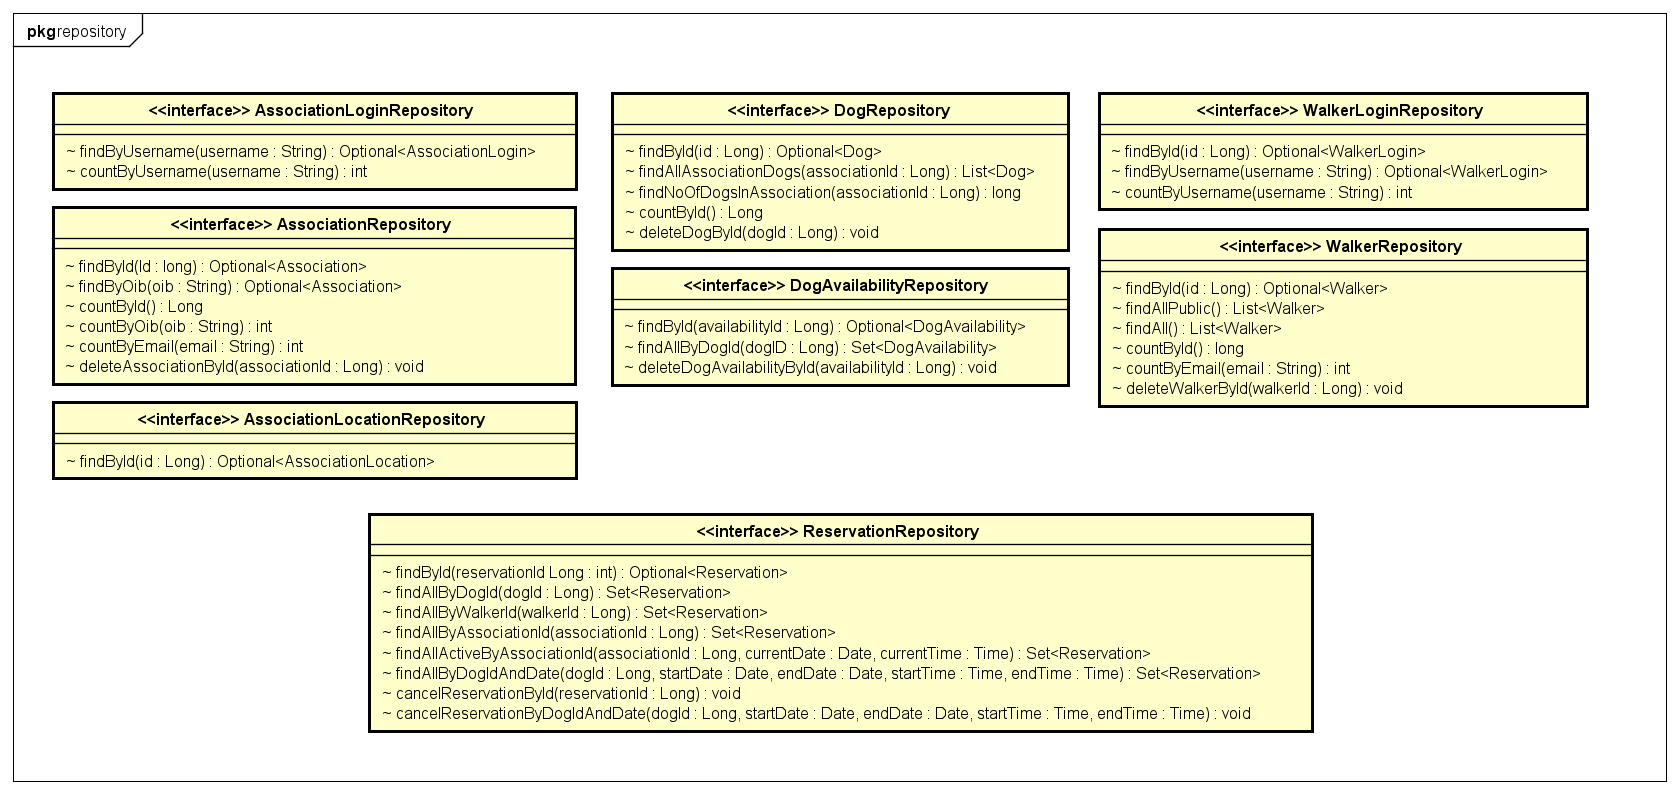
\includegraphics[scale=0.34]{dijagrami/classdiagram-repository.png}
    			    \centering
    			    \caption{Dijagram spremišnih razreda}
    			    \label{fig:classdiagram-repository}
		    \end{figure}
		    
		    
		    
		     \begin{figure}[H]
    			    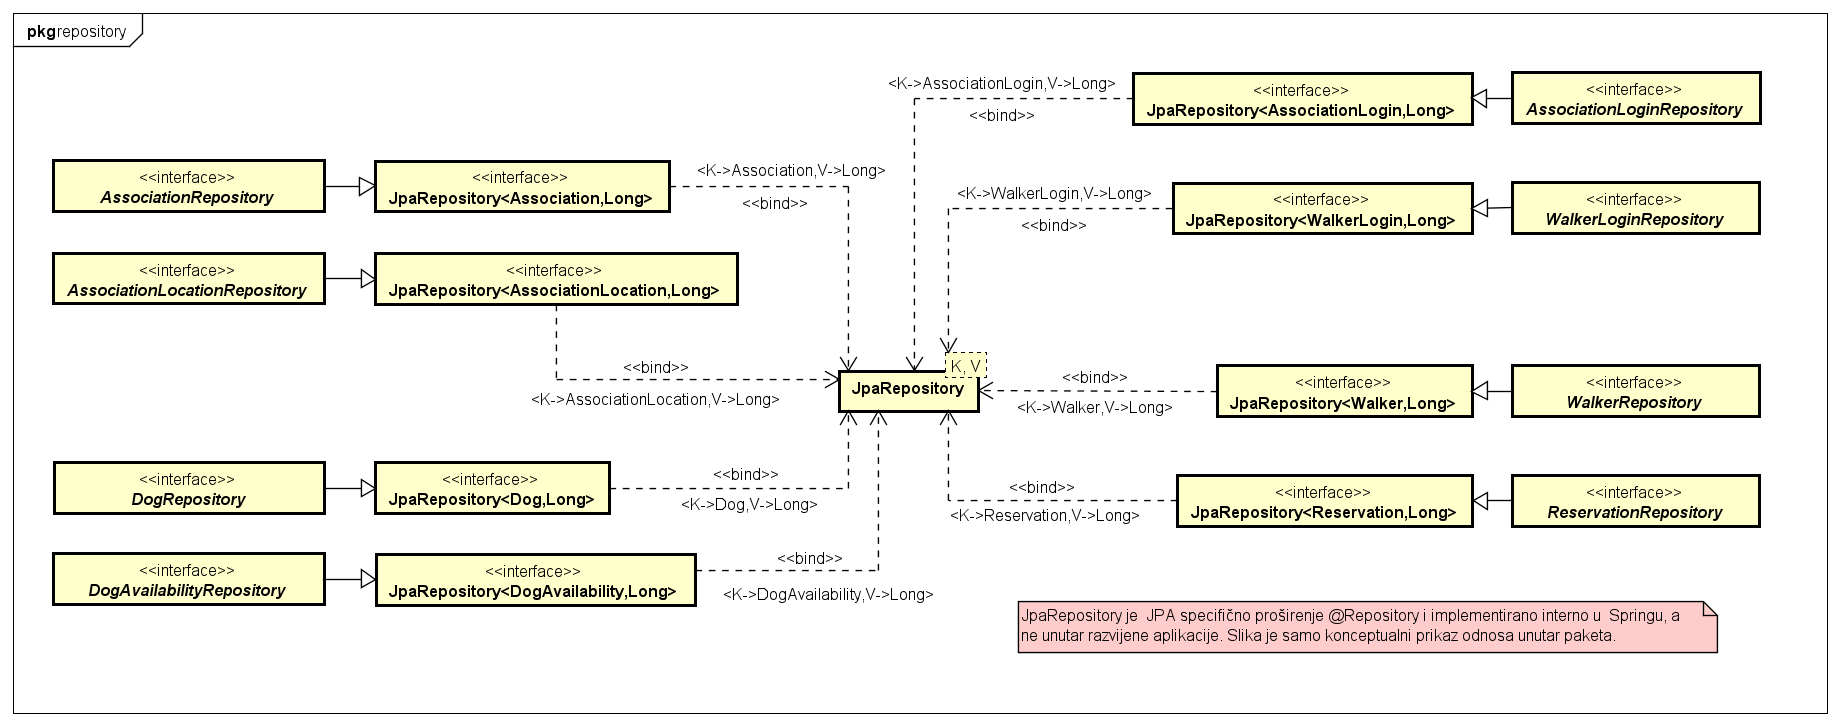
\includegraphics[scale=0.31]{dijagrami/classdiagram-repository-jpa.png}
    			    \centering
    			    \caption{Nasljeđivanje JPA repozitorija}
    			    \label{fig:classdiagram-repository-jpa}
		    \end{figure}
		    
		    \bigskip
		    \noindent Paket \textit{service} sadrži sučelja koja definiraju funkcionalnosti servisnog sloja. Ona se ostvaruju u potpaketu \textit{impl}. Implementacijske klase sadrže reference na potrebne repozitorije kako bi mogle dohvaćati i spremati podatke te manipulirati njima.
		    
		    \begin{figure}[H]
    			    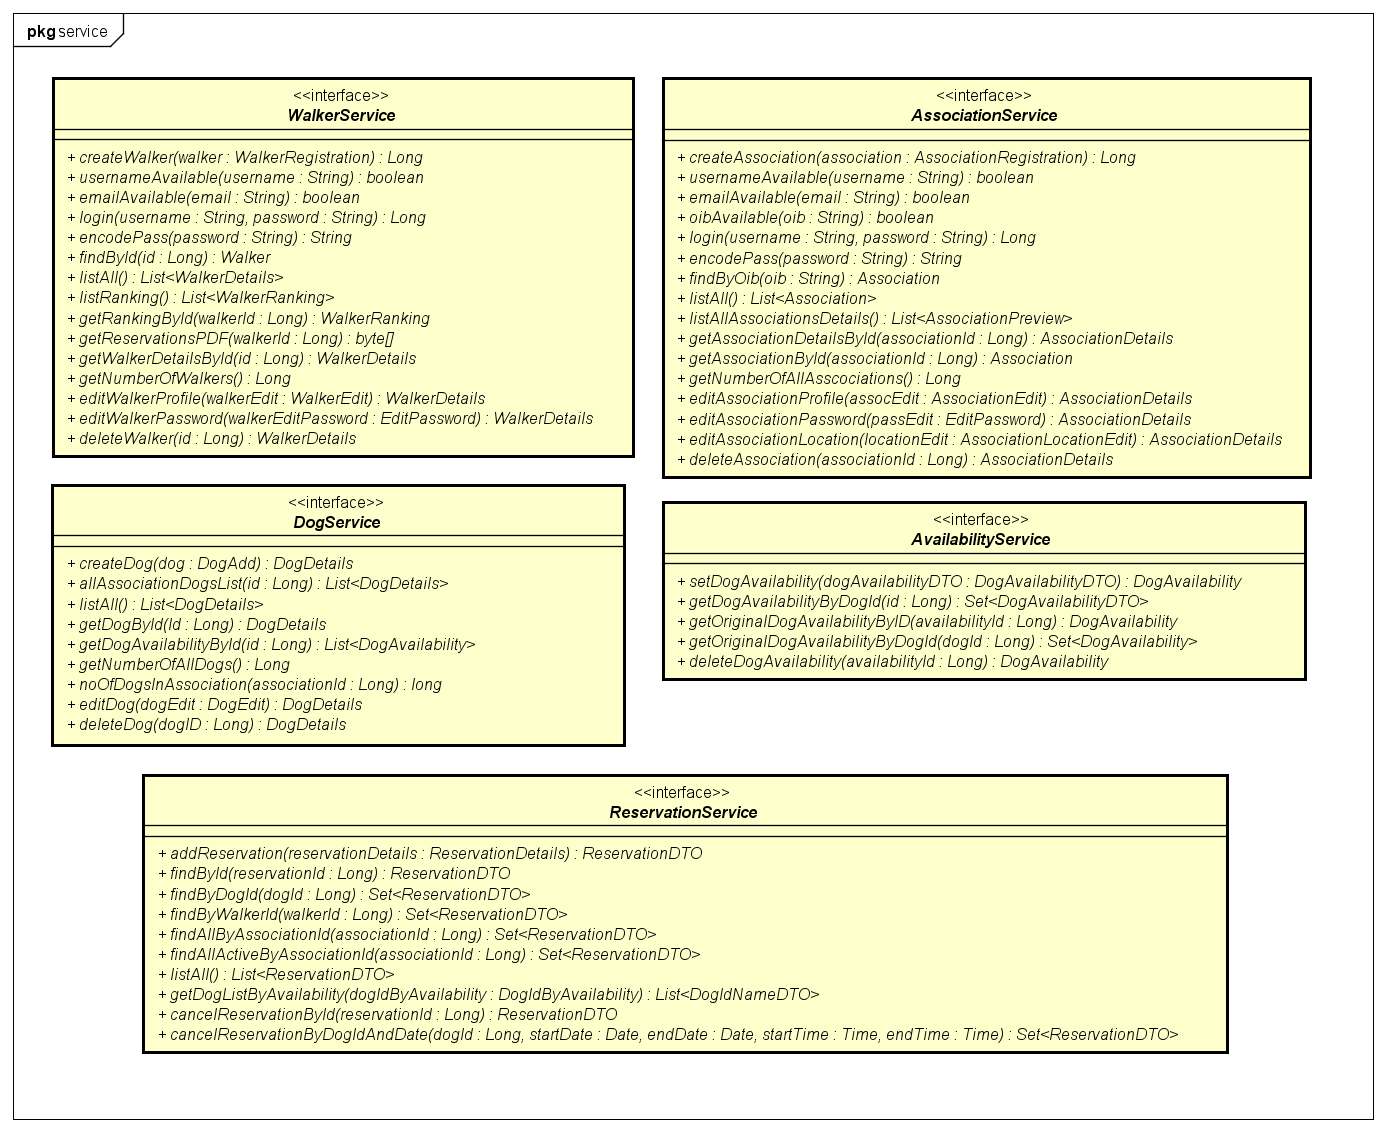
\includegraphics[scale=0.27]{dijagrami/classdiagram-service.png}
    			    \centering
    			    \caption{Dijagram servisnih sučelja}
    			    \label{fig:classdiagram-service}
		    \end{figure}
		    
		    \begin{figure}[H]
    			    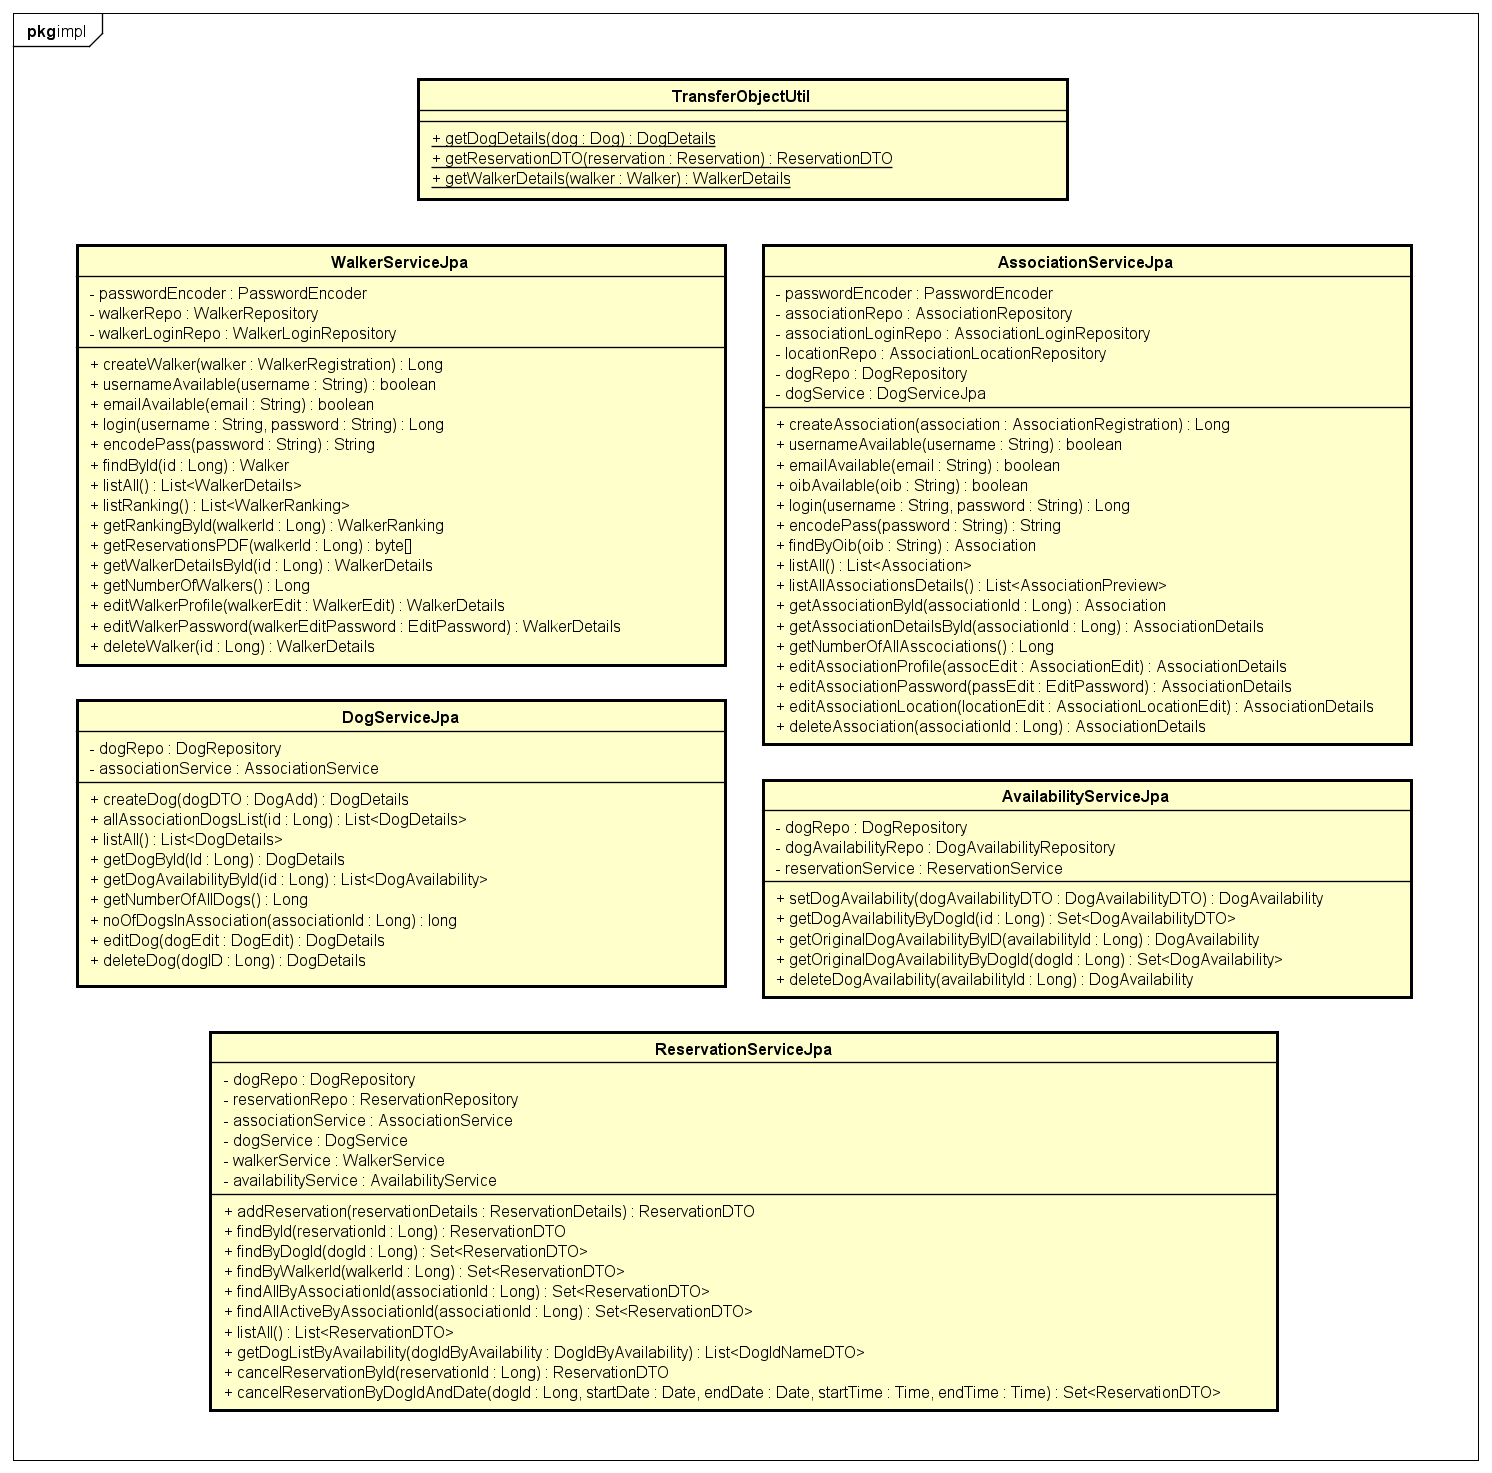
\includegraphics[scale=0.32]{dijagrami/classdiagram-service-impl.png}
    			    \centering
    			    \caption{Dijagram razreda implementacije servisnih sučelja}
    			    \label{fig:classdiagram-service-impl}
		    \end{figure}
		    
		    \noindent Razredi paketa \textit{rest} komuniciraju s \textit{frontend} stranom razvijenog sustava i nazivaju se i kontrolerima. Razmijenjuju informacije u formatu JSON i odgovarajućim HTTP status kodom. Za formatiranje odgovora koriste se razredima paketa DTO (engl. \textit{Data Transfer Object}). Sadrže reference na servisna sučelja kojima dohvaćaju obrađene podatke ili ih šalju na obradu.
		    
		    \bigskip
		    
		    \begin{figure}[H]
    			    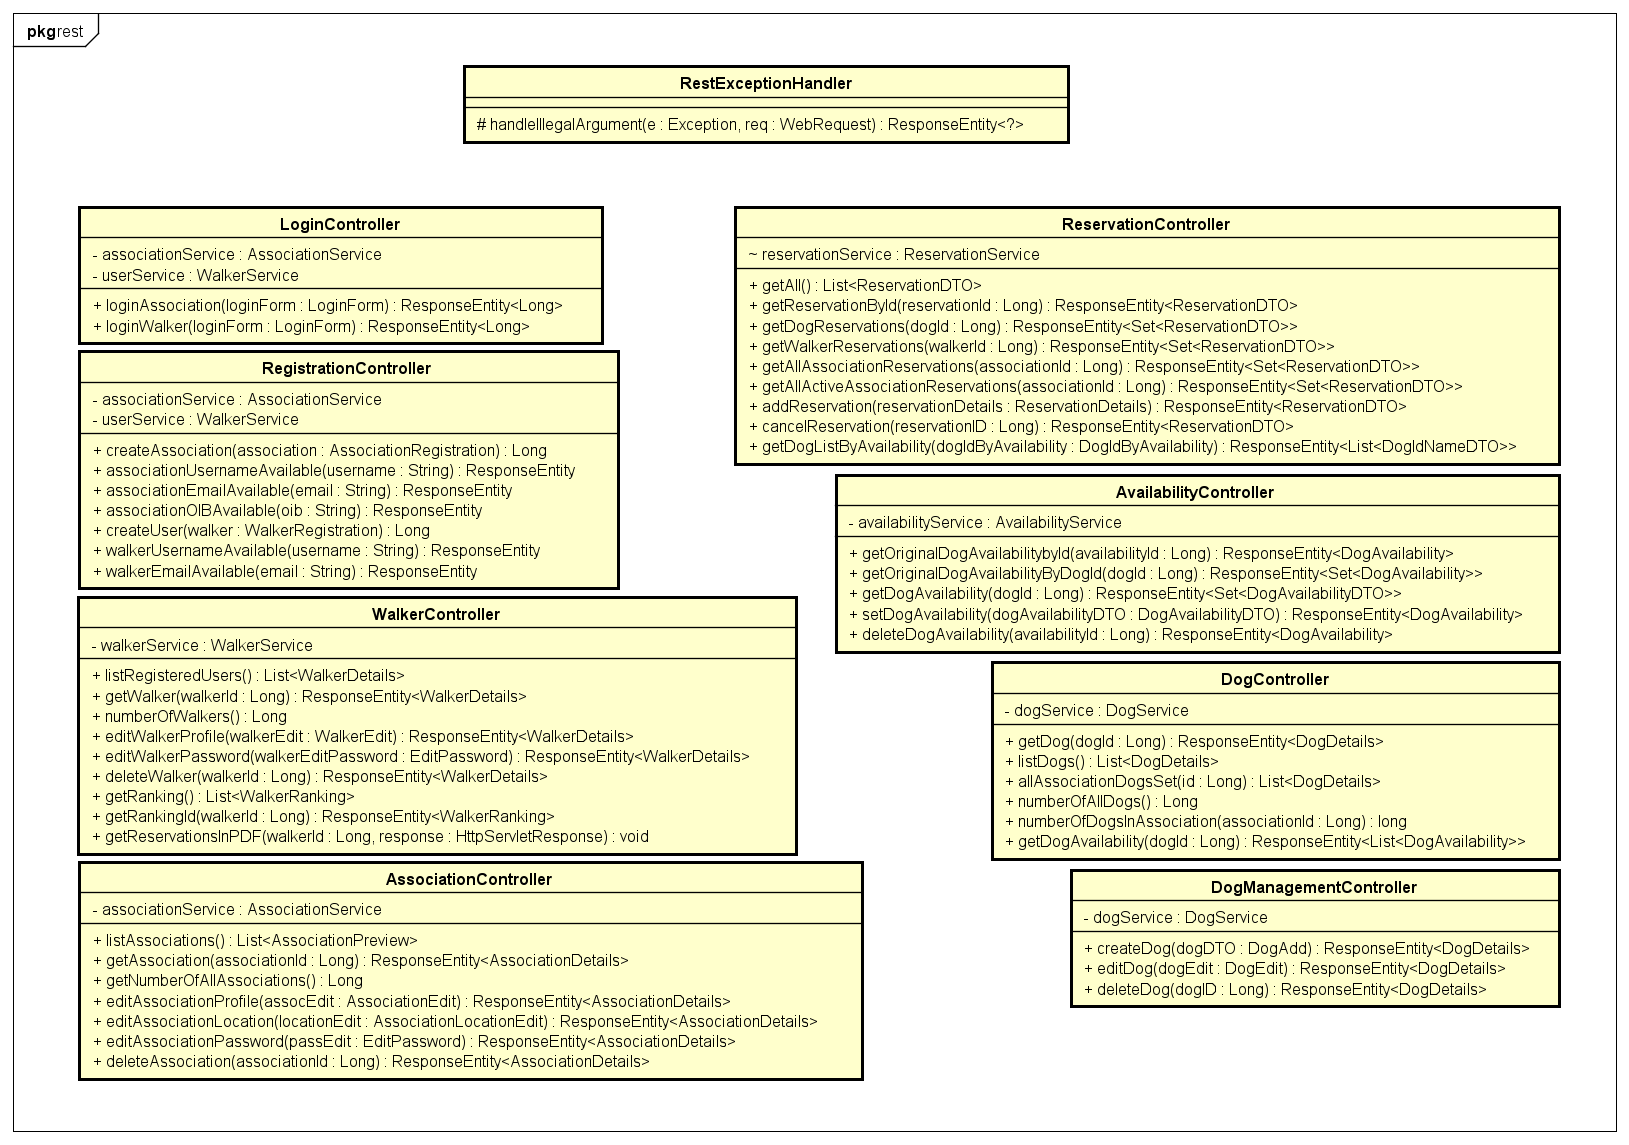
\includegraphics[scale=0.35]{dijagrami/classdiagram-rest.png}
    			    \centering
    			    \caption{Dijagram razreda kontrolera}
    			    \label{fig:classdiagram-rest}
		    \end{figure}
		    
		    \bigskip
		    
		    \noindent Na slici \ref{fig:classdiagram-doggo} moguće je vidjeti ishodišni razred cijele aplikacije \textit{DogGoApplication} i razred konfiguracije dozvoljenih HTTP zahtjeva u aplikaciji koji nasljeđuje već gotovi razred Spring razvojnog okvira \textit{WebMvcConfigurer}.
		    
		    \bigskip
		    
		     \begin{figure}[H]
    			    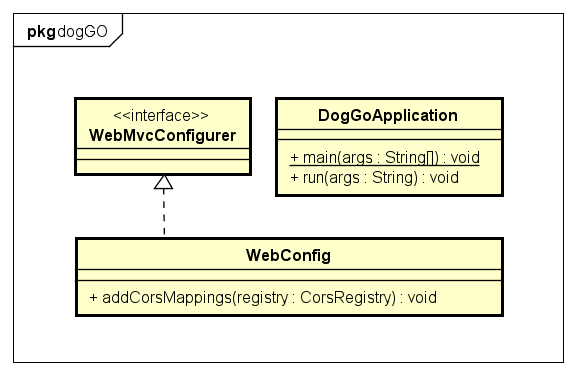
\includegraphics[scale=0.35]{dijagrami/classdiagram-doggo.png}
    			    \centering
    			    \caption{Ishodišni paket aplikacije}
    			    \label{fig:classdiagram-doggo}
		    \end{figure}
		    
		    \begin{figure}[H]
    			    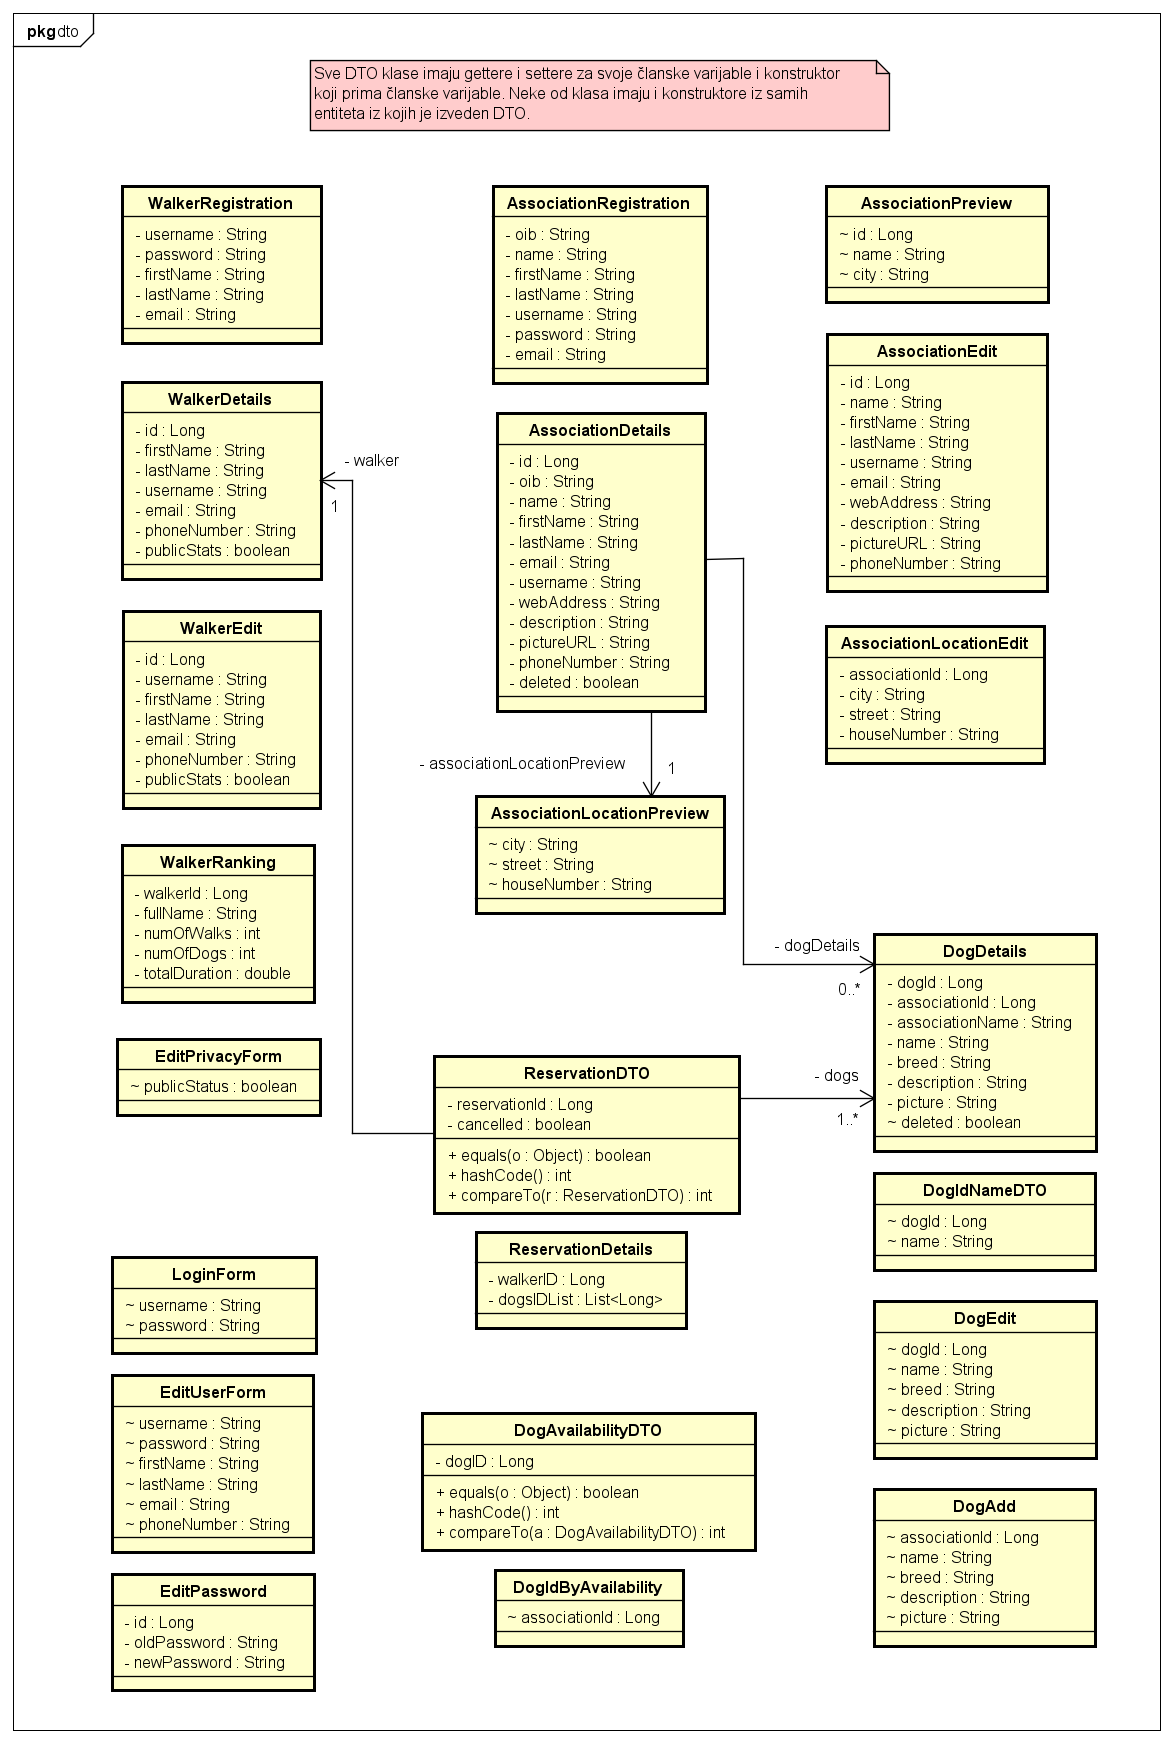
\includegraphics[scale=0.47]{dijagrami/classdiagram-rest-dto.png}
    			    \centering
    			    \caption{Dijagram razreda objekata prijenosa podataka}
    			    \label{fig:classdiagram-rest-dto}
		    \end{figure}
			
			\eject
		
		\section{Dijagram stanja}
			
			Dijagram stanja prikazuje stanja objekata te prijelaze iz jednog u drugo stanje na temelju događaja.
Na slici \ref{fig:states} je prikazan dijagram stanja za registriranog šetača. 
Neregistriranom korisniku se prikazuje naslovna stranica. Od tamo, korisnik može pregledati javnu statistiku te može dobiti uvid u sve registrirane udruge i njihove profile gdje su prikazane informacije o njima i svim njihovim psima.
Nakon prijave korisnika kao šetača, korisnik dobiva mogućnost rezervacije šetnje odabranog psa u slobodnom terminu. Na stranici „Moj profil“ korisnik može urediti osobne podatke, pregledati kalendar rezerviranih šetnji te u obliku pdf-a skinuti vlastiti raspored nadolazećih šetnji te obrisati svoj profil.

    \begin{figure}[H]
    			    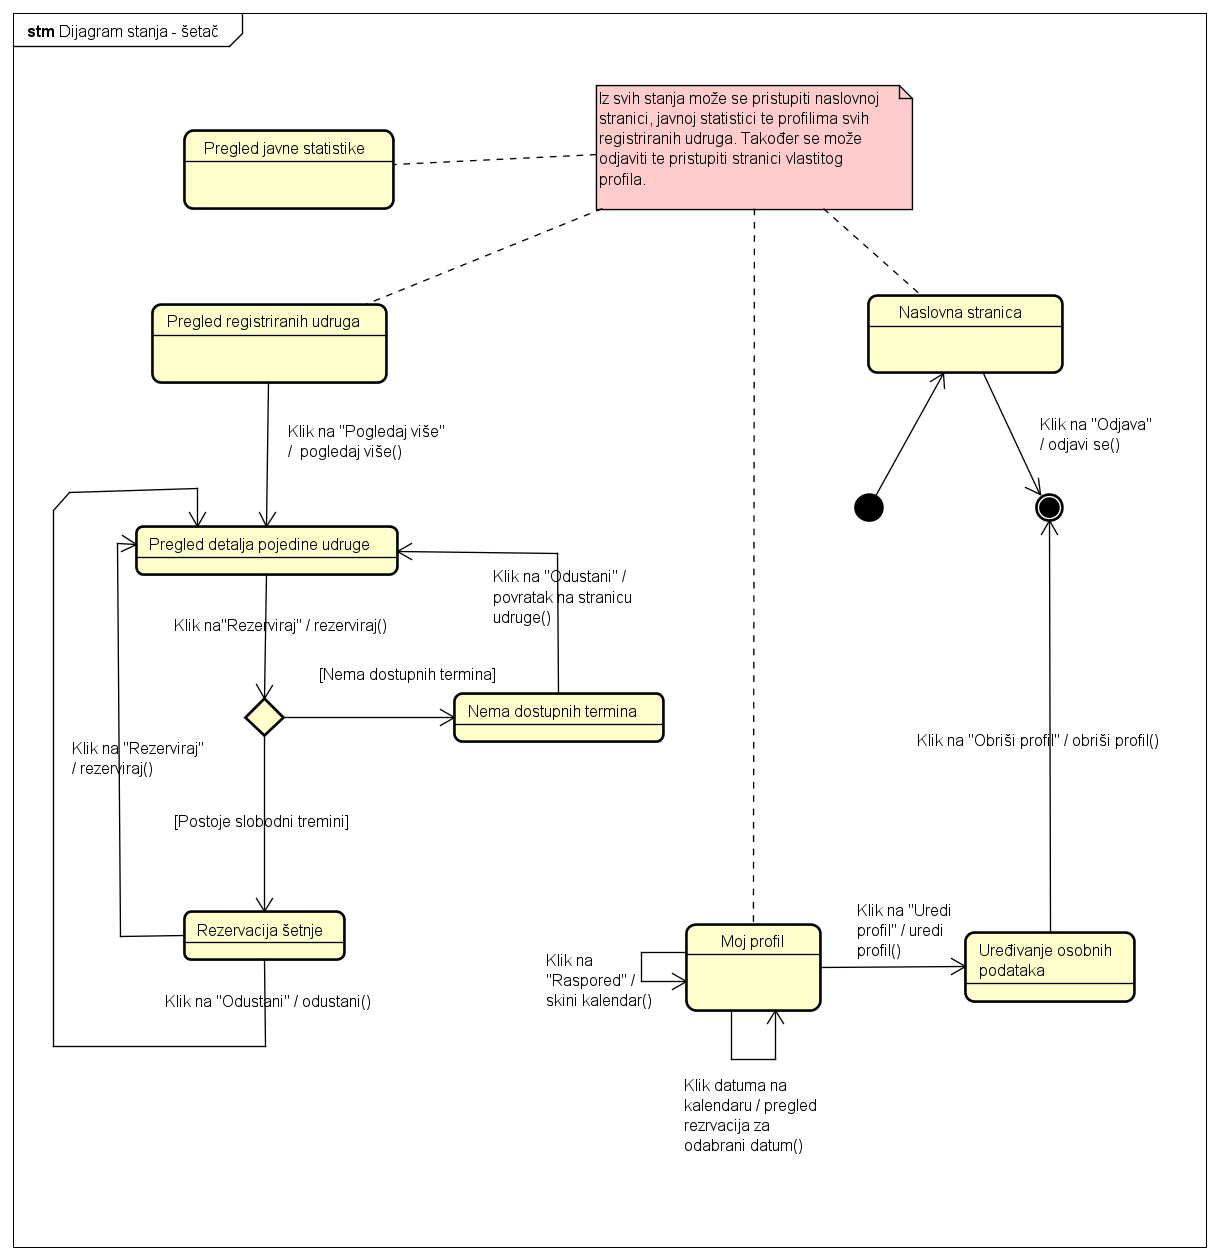
\includegraphics[scale=0.45]{dijagrami/Dijagram_stanja-setac.png}
    			    \centering
    			    \caption{Dijagram stanja}
    			    \label{fig:states}
		    \end{figure}
			
		
			\eject 
		
		\section{Dijagram aktivnosti}
			
			\begin{figure}[H]
			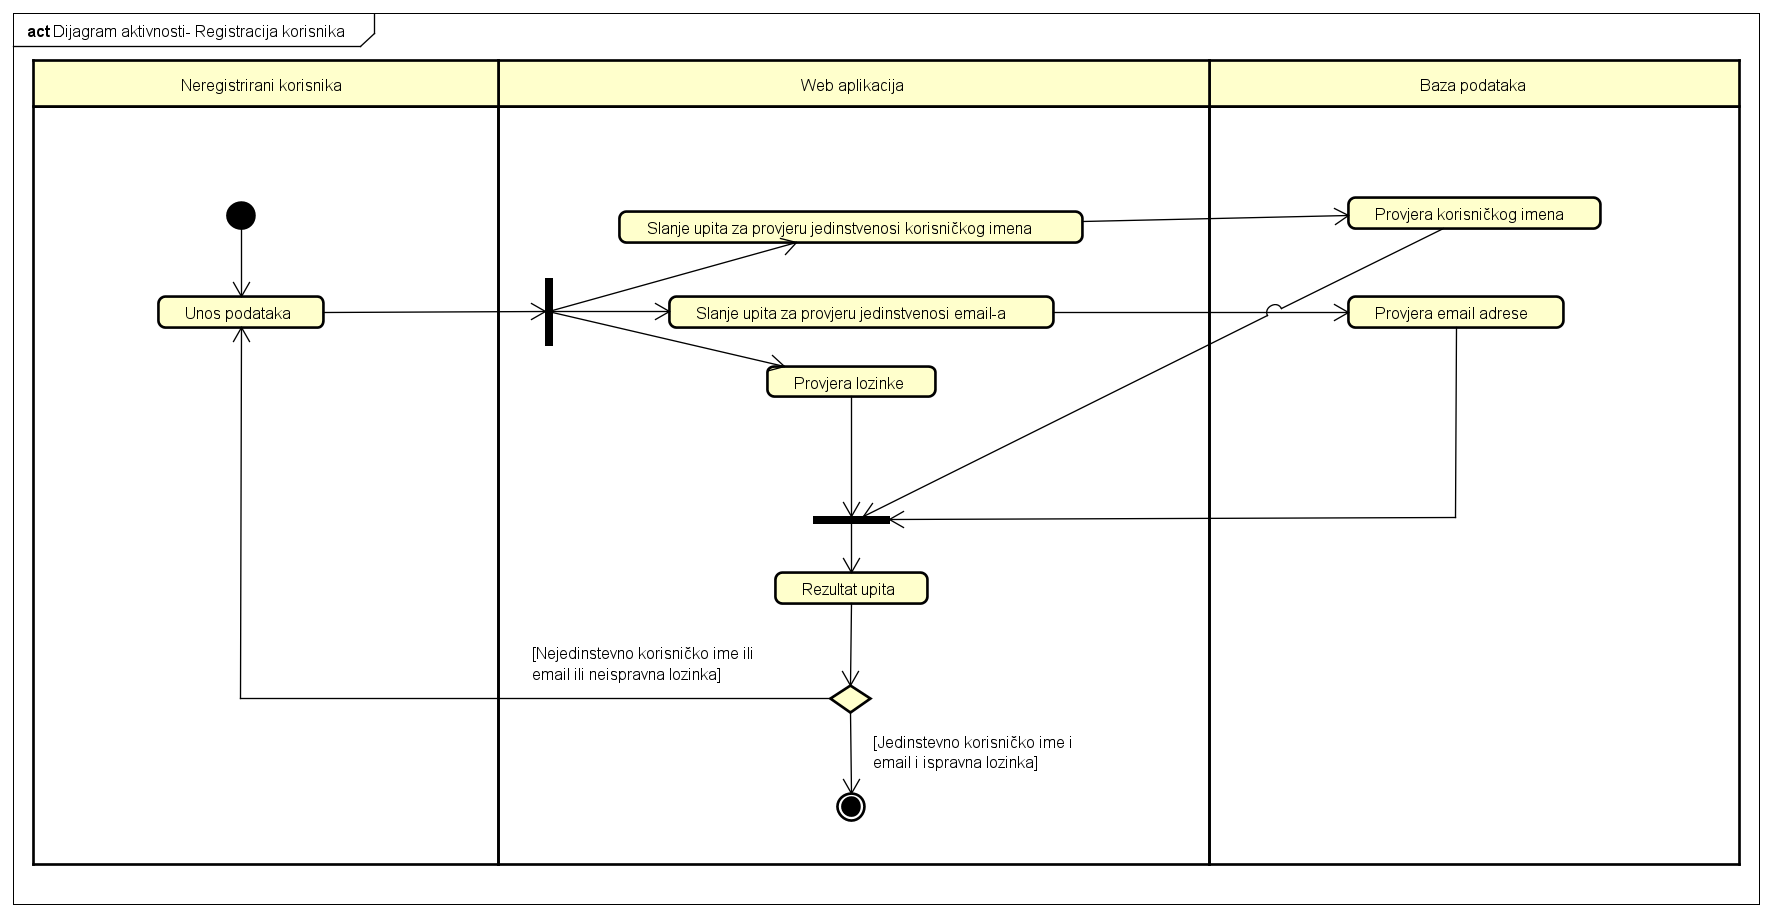
\includegraphics[scale=0.3]{dijagrami/Dijagram_aktivnosti-Registracija_korisnika.png}
			\centering
			\caption{Dijagram aktivnosti za registraciju korisnika}
			\label{fig:activity_diagram_1}
		\end{figure}	

		\begin{figure}[H]
			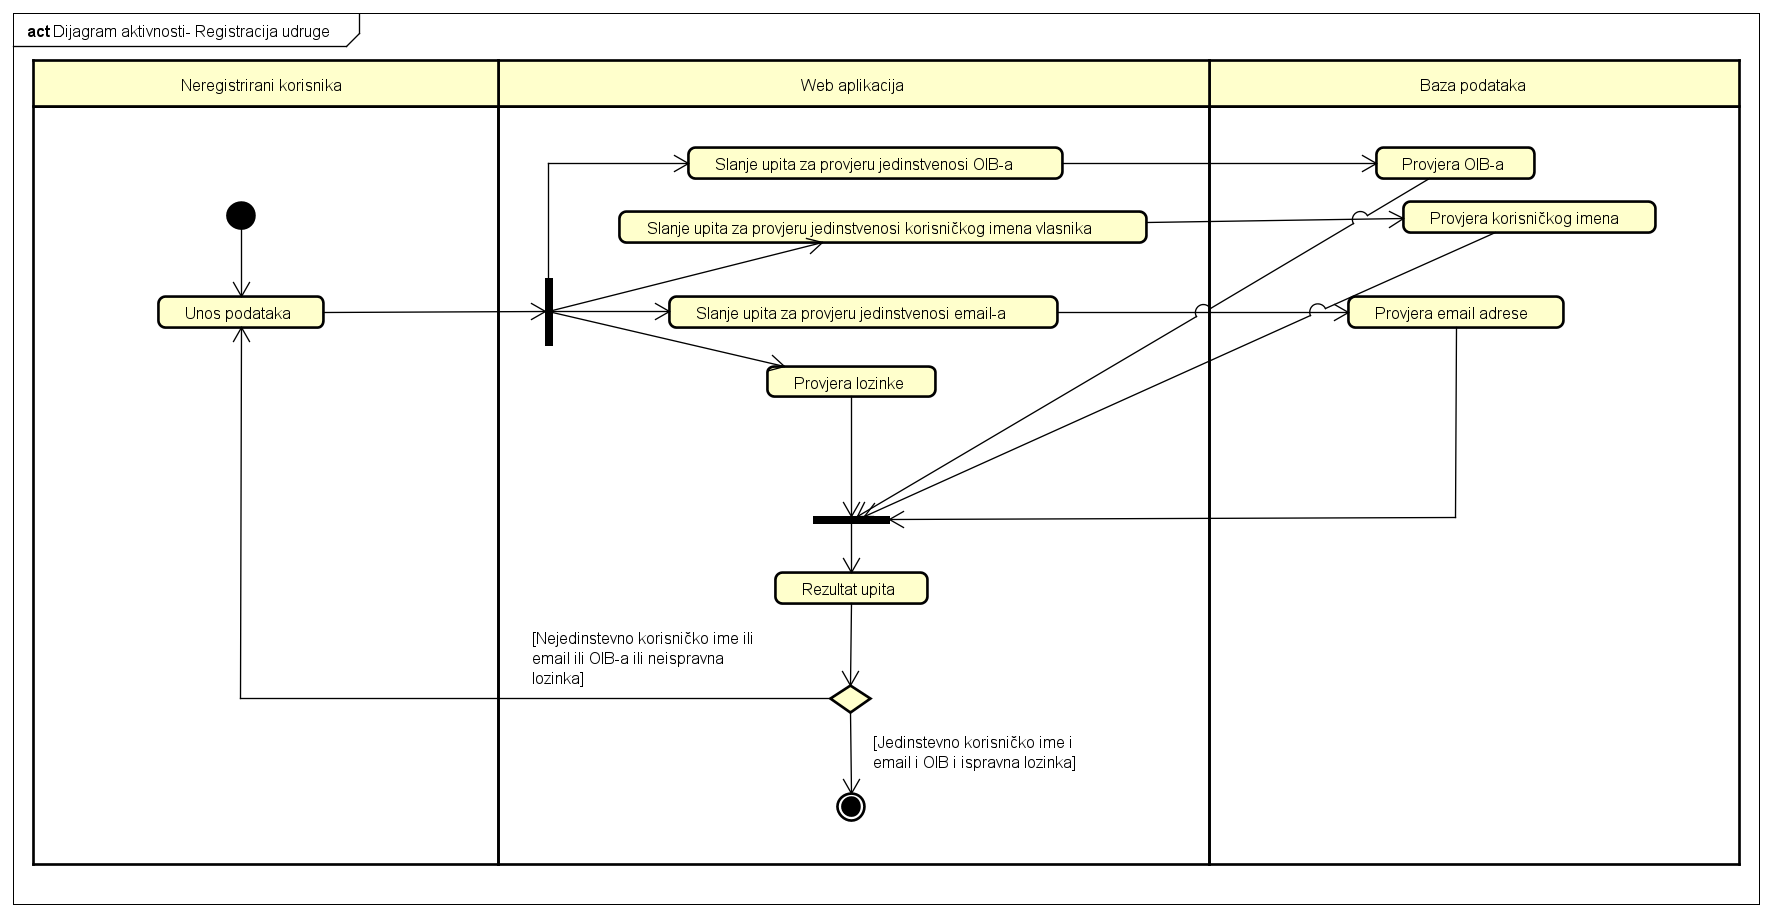
\includegraphics[scale=0.3]{dijagrami/Dijagram_aktivnosti-Registracija_udruge.png}
			\centering
			\caption{Dijagram aktivnosti za registraciju udruga}
			\label{fig:activity_diagram_2}
		\end{figure}	

		\begin{figure}[H]
			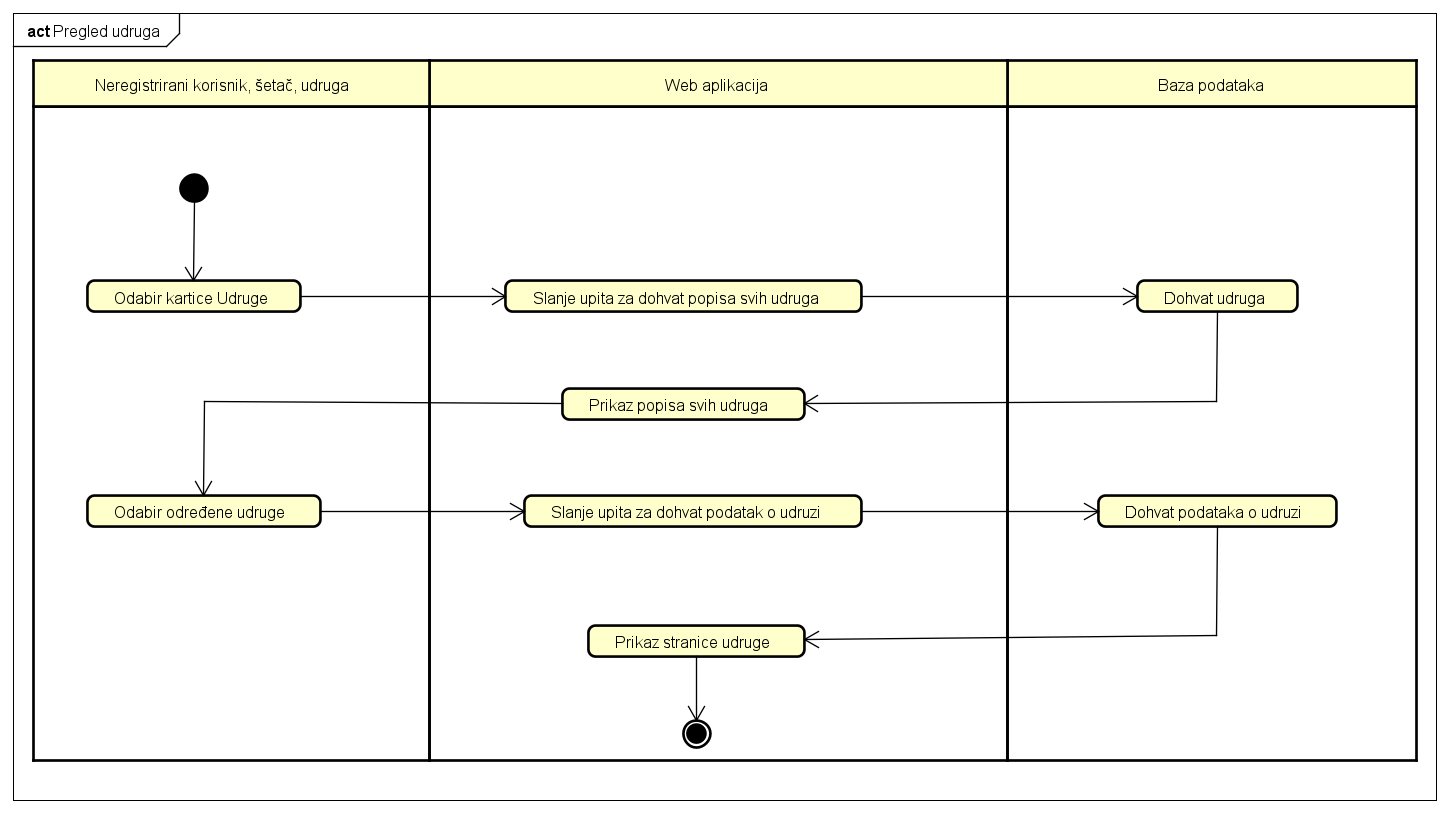
\includegraphics[scale=0.4]{dijagrami/Pregled_udruga.png}
			\centering
			\caption{Dijagram aktivnosti za pregled svih udruga}
			\label{fig:activity_diagram_3}
		\end{figure}

		\begin{figure}[H]
			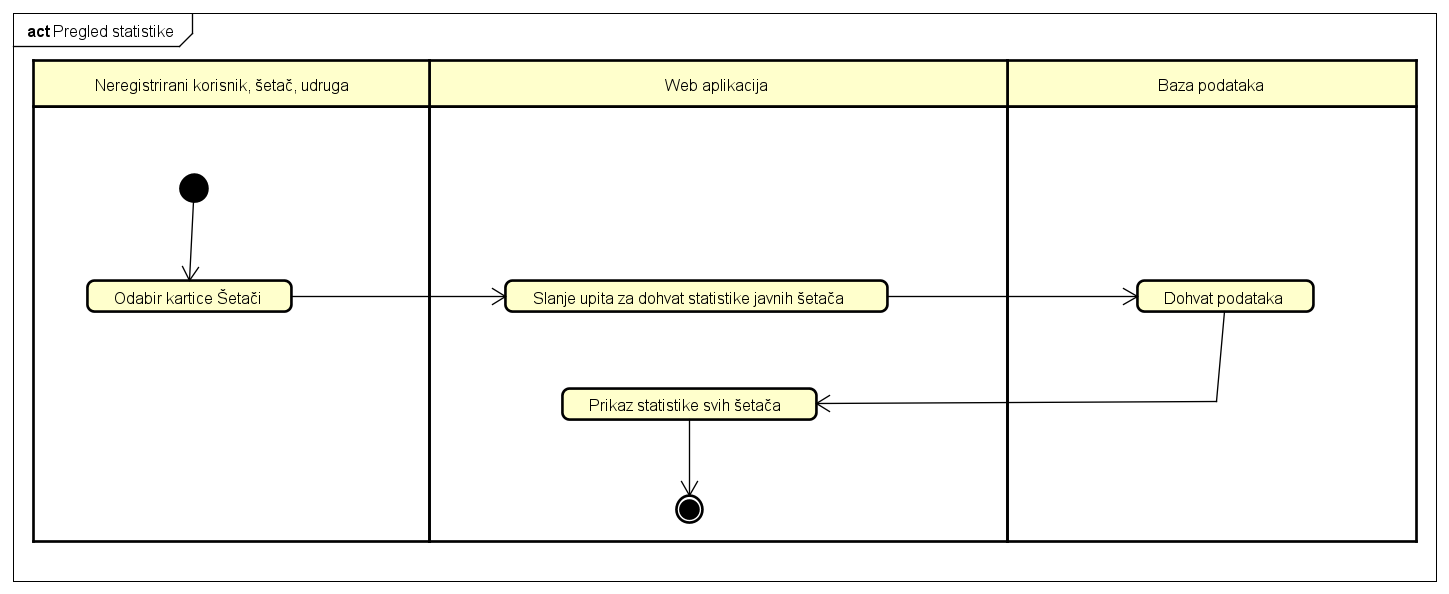
\includegraphics[scale=0.4]{dijagrami/Pregled_statistike.png}
			\centering
			\caption{Dijagram aktivnosti za pregled statistike šetača}
			\label{fig:activity_diagram_4}
		\end{figure}


		\begin{figure}[H]
			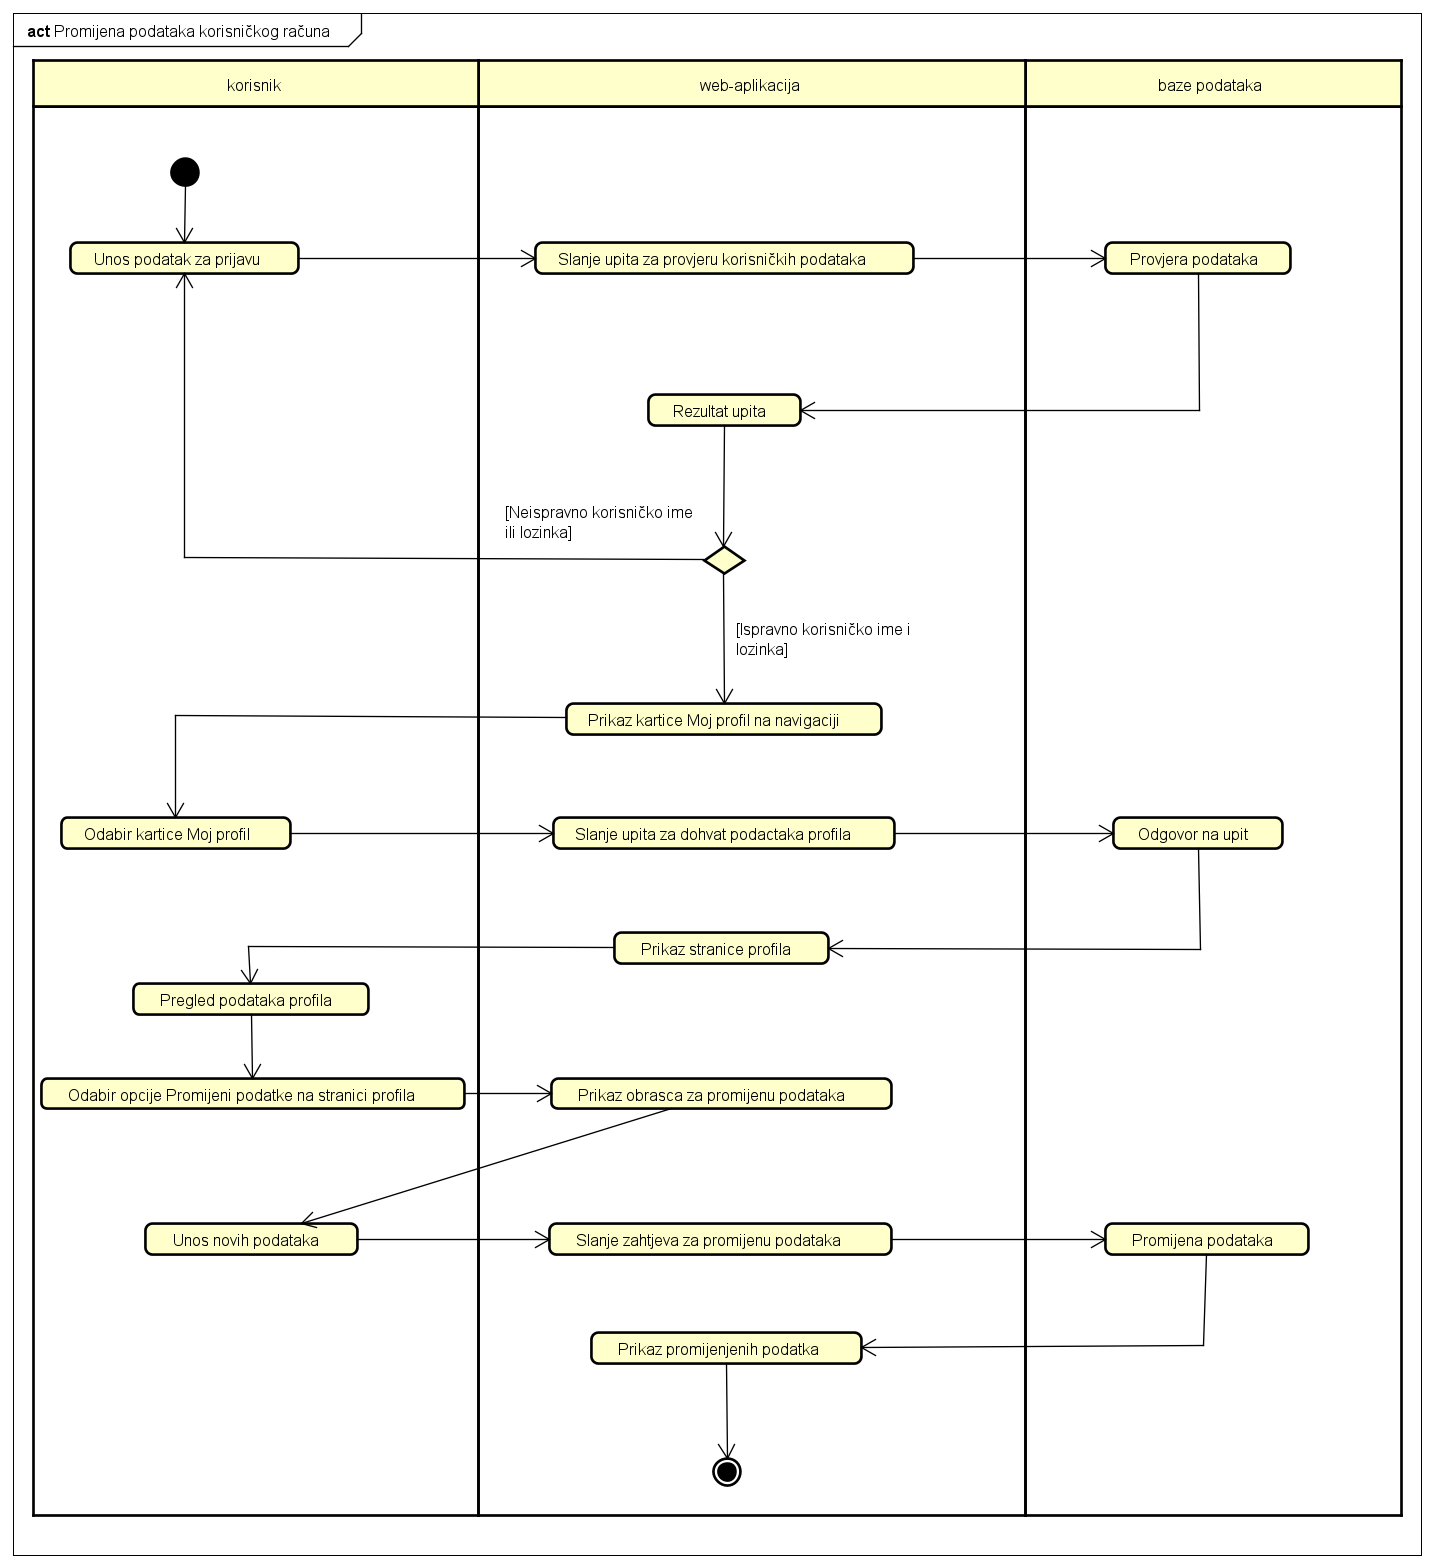
\includegraphics[scale=0.4]{dijagrami/Promijena_podataka_korisnickog_racuna.png}
			\centering
			\caption{Dijagram aktivnosti za promjenu podataka korisničkog računa}
			\label{fig:activity_diagram_5}
		\end{figure}


		\begin{figure}[H]
			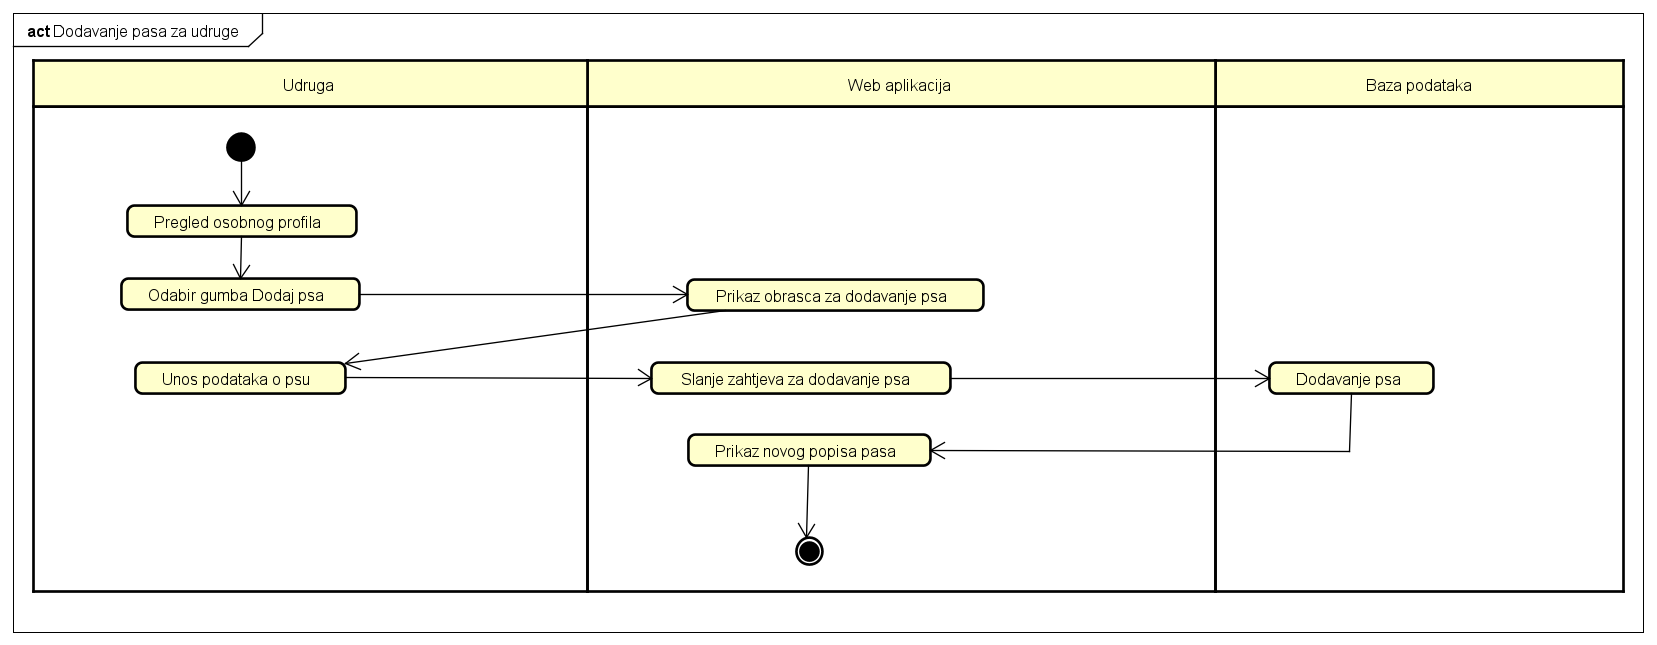
\includegraphics[scale=0.4]{dijagrami/Dodavanje_pasa_za_udruge.png}
			\centering
			\caption{Dijagram aktivnosti za dodavanje pasa kod udruga}
			\label{fig:activity_diagram_6}
		\end{figure}

		\begin{figure}[H]
			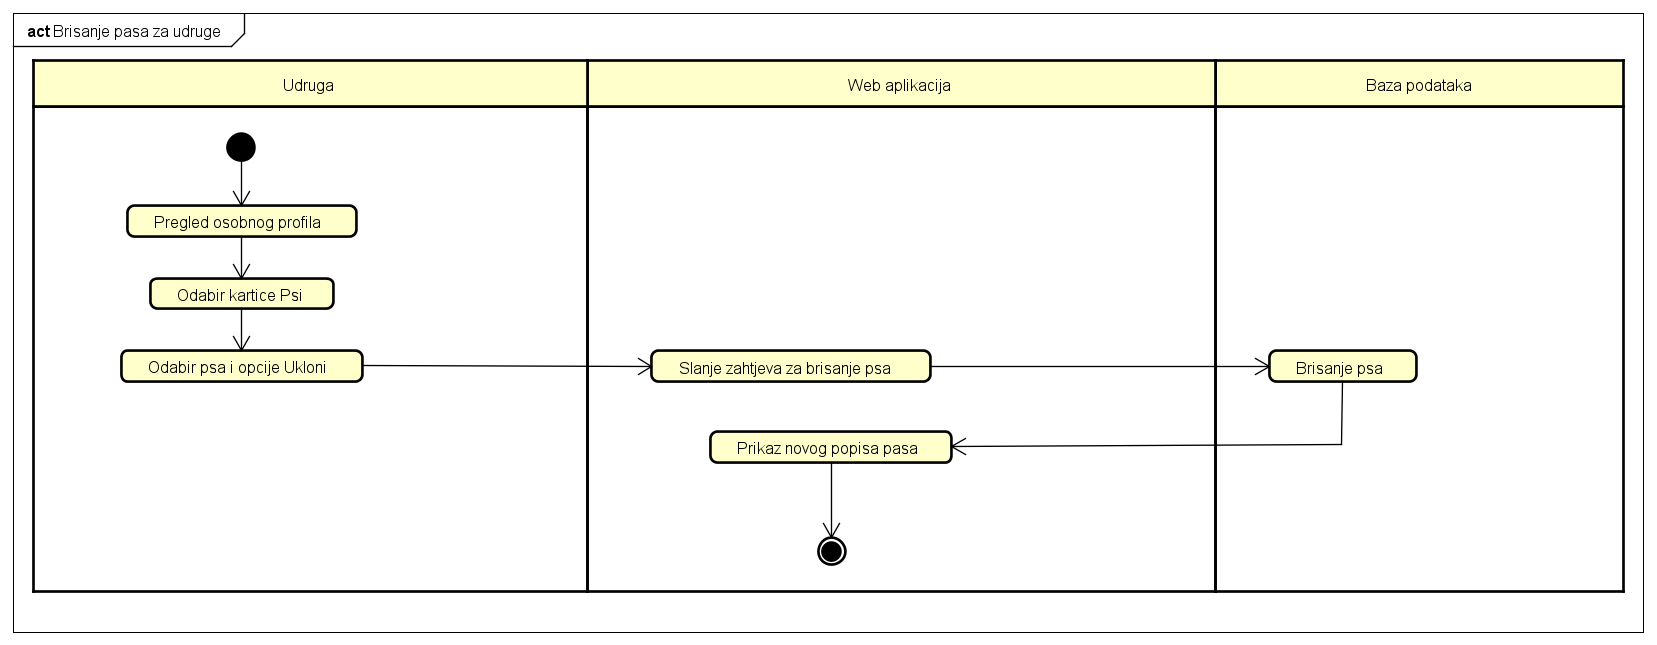
\includegraphics[scale=0.4]{dijagrami/Brisanje_pasa_za_udruge.png}
			\centering
			\caption{Dijagram aktivnosti za brisanje pasa kod udruga}
			\label{fig:activity_diagram_7}
		\end{figure}

		\begin{figure}[H]
			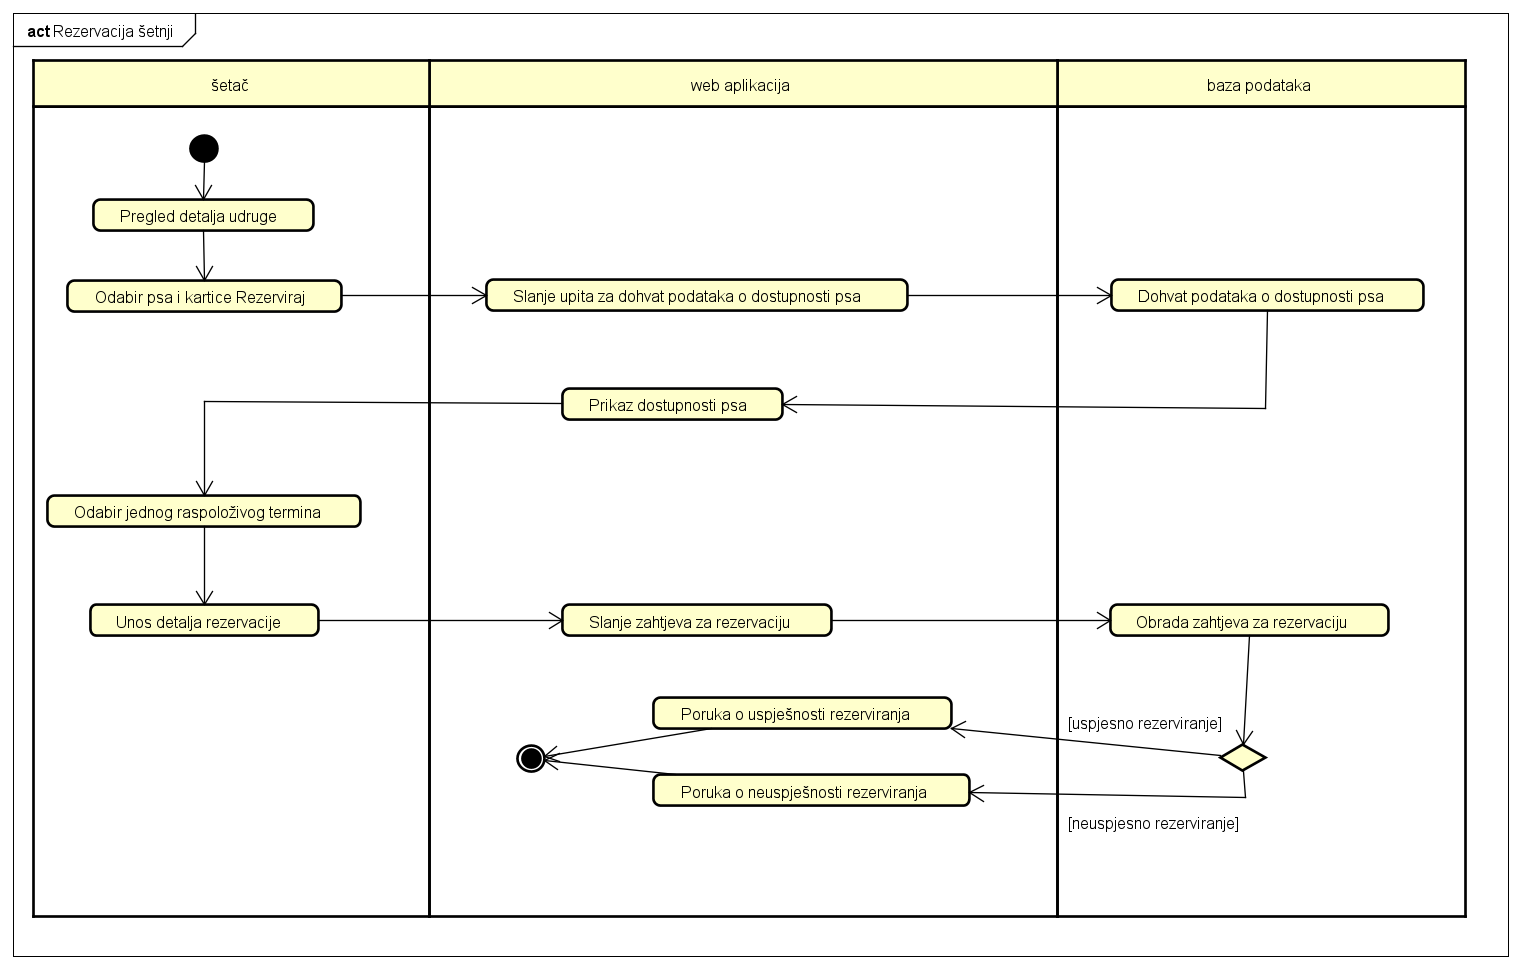
\includegraphics[scale=0.4]{dijagrami/Rezervacija_setnji.png}
			\centering
			\caption{Dijagram aktivnosti za rezervaciju šetnji}
			\label{fig:activity_diagram_8}
		\end{figure}

		\begin{figure}[H]
			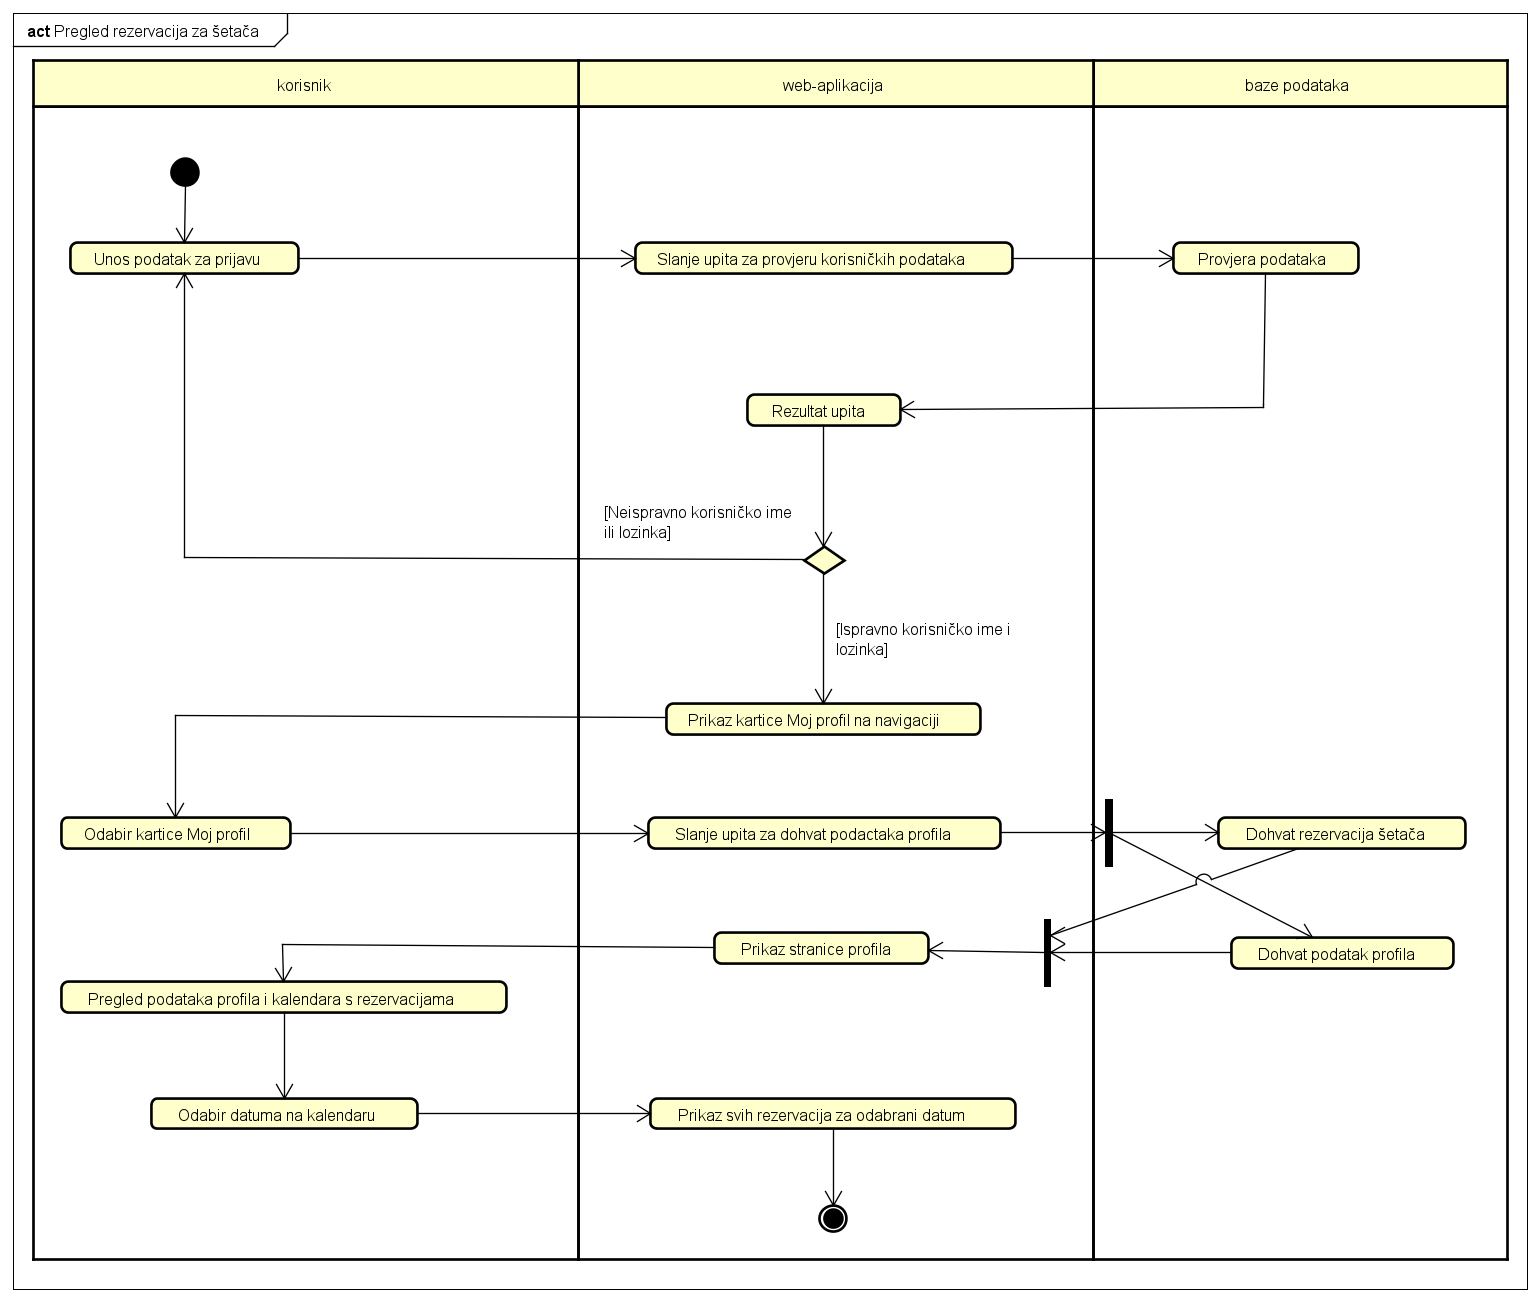
\includegraphics[scale=0.4]{dijagrami/Pregled_rezervacija_za_setaca.png}
			\centering
			\caption{Dijagram aktivnosti za pregled rezervacija šetača}
			\label{fig:activity_diagram_9}
		\end{figure}

		\begin{figure}[H]
			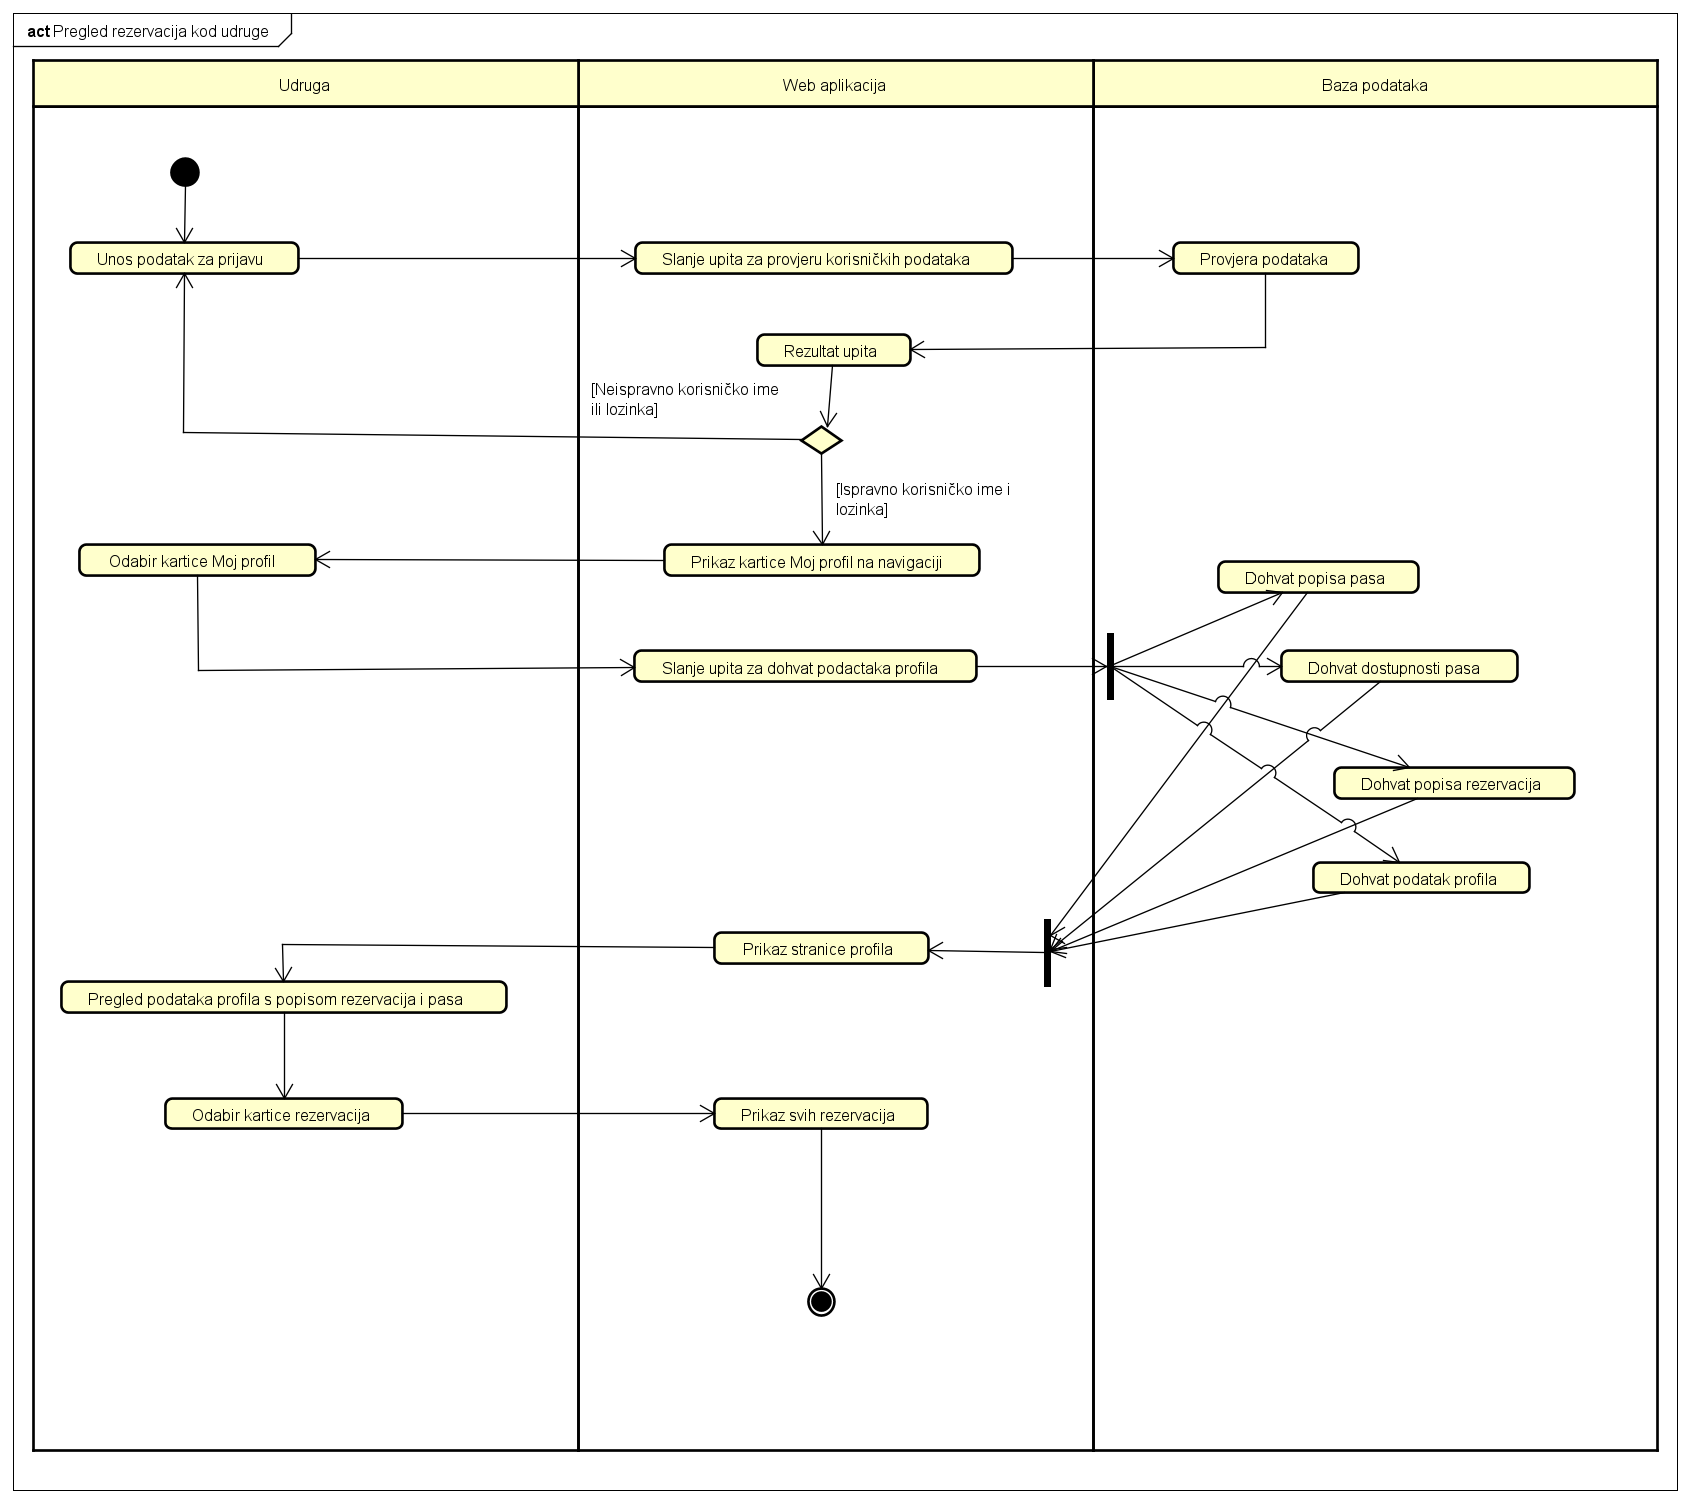
\includegraphics[scale=0.4]{dijagrami/Pregled_rezervacija_kod_udruge.png}
			\centering
			\caption{Dijagram aktivnosti za pregled rezervacija udruge}
			\label{fig:activity_diagram_10}
		\end{figure}

		\begin{figure}[H]
			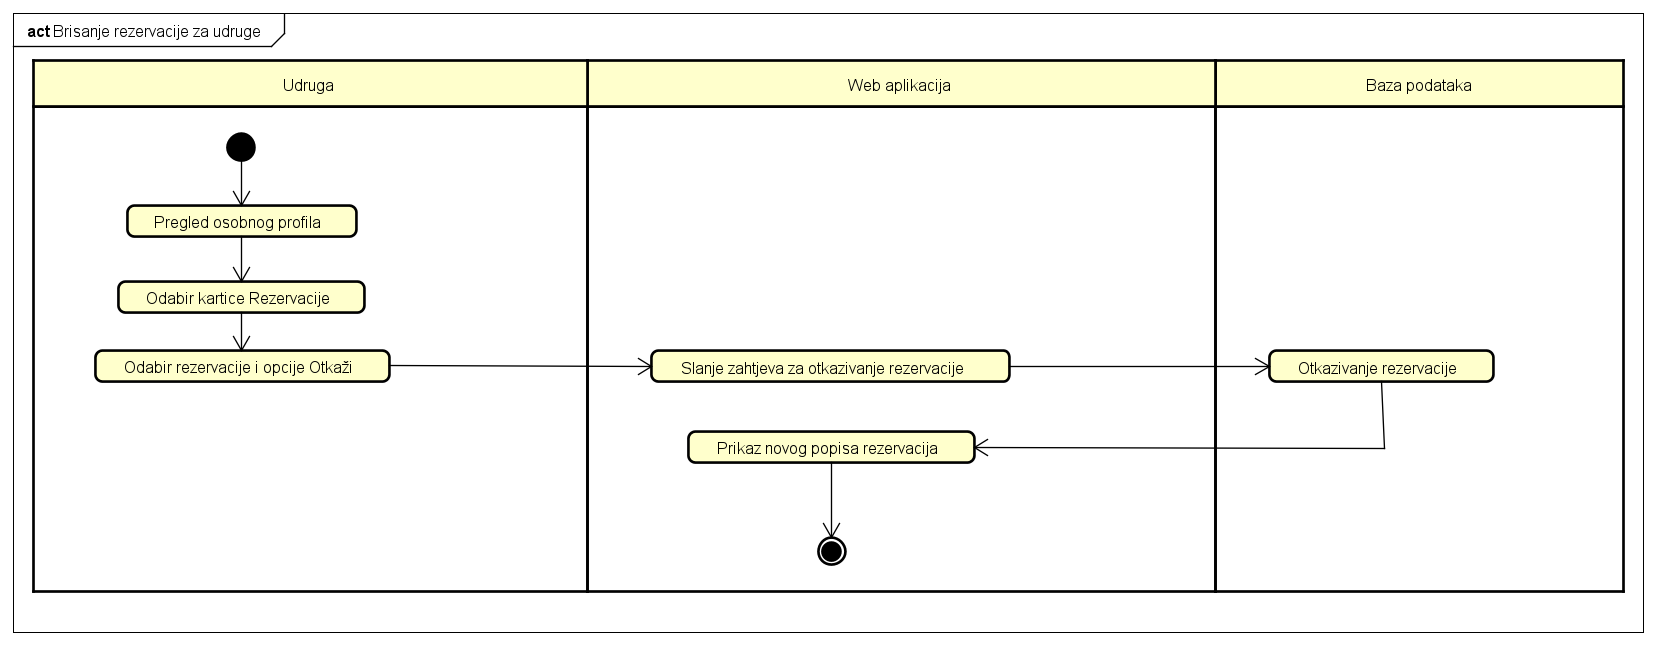
\includegraphics[scale=0.4]{dijagrami/Brisanje_rezervacije_za_udruge.png}
			\centering
			\caption{Dijagram aktivnosti za brisanje rezervacije kod udruge}
			\label{fig:activity_diagram_11}
		\end{figure}

		\begin{figure}[H]
			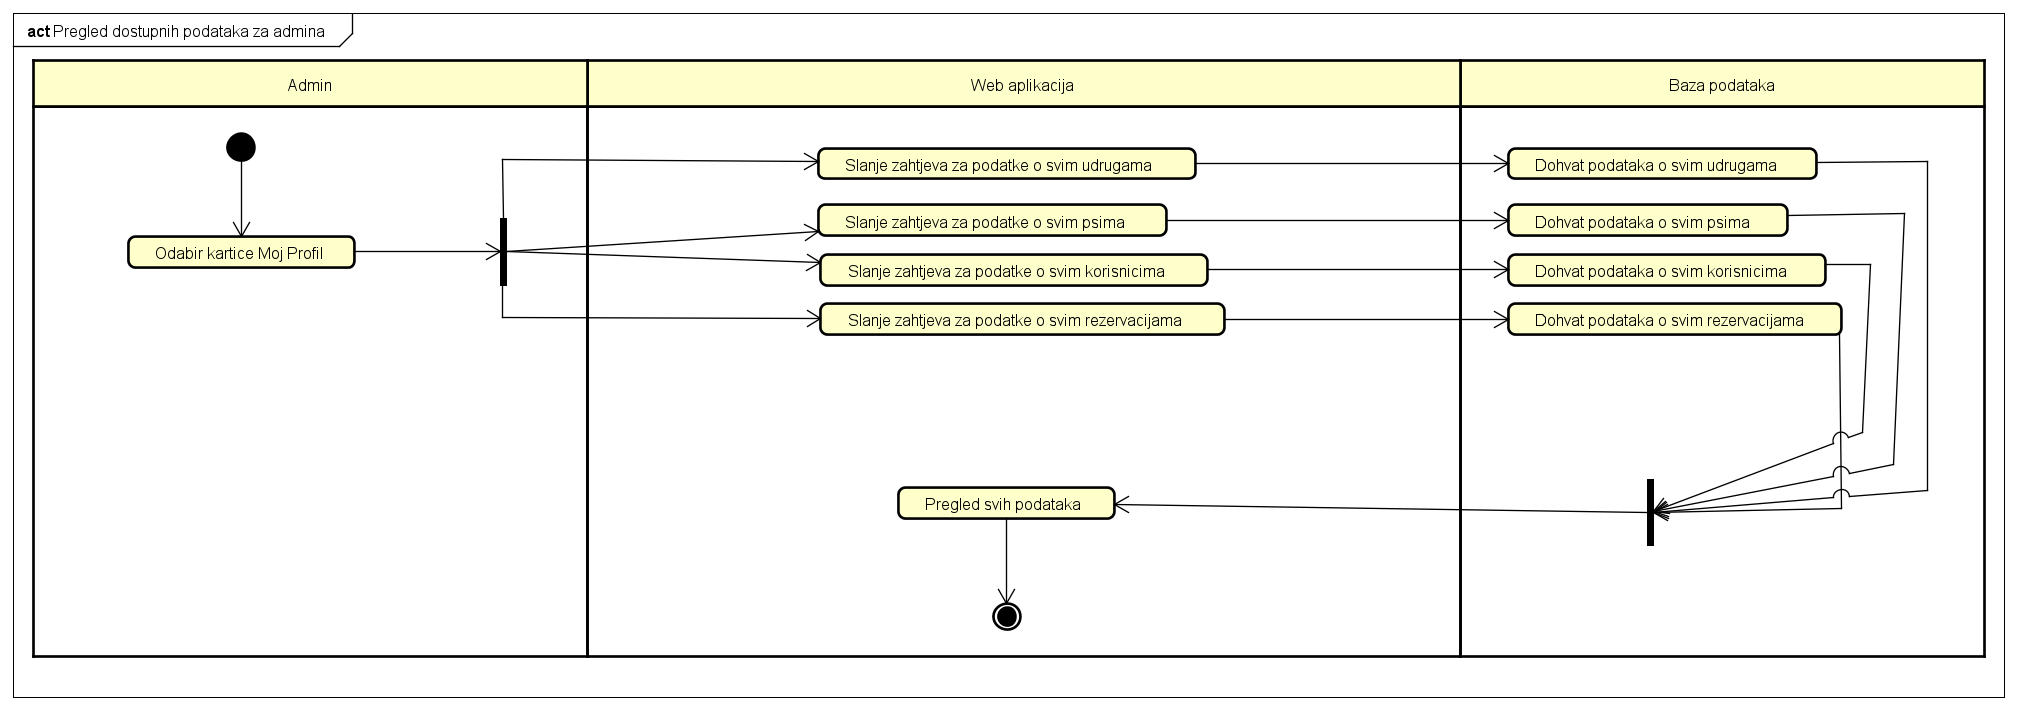
\includegraphics[scale=0.3]{dijagrami/Pregled_dostupnih_podataka_za_admina.png}
			\centering
			\caption{Dijagram aktivnosti za pregled dostupnih podataka za admina}
			\label{fig:activity_diagram_12}
		\end{figure}
			
			\eject
		\section{Dijagram komponenti}
		Dijagram komponenti je strukturni, statički UML dijagram koji vizualizira organizaciju i međuovisnost komponenata aplikacije, s naglaskom na implementaciju sustava, stoga je koristan za stjecanje okvirne ideje o implementaciji sustava, bez ulaženja u prevelike detalje.
		 
		U prikazanom dijagramu našu aplikaciju smo podijelili na 4 glavne komponente:komponentu React view, koji je zadužen za de-facto upravljanje cijelom aplikacijom, komponentu frontend logike, zaduženu za dohvat odgovarajućih HTML, CSS i .js datoteka, komponentu backend logike, zaduženu za dohvat i obradu podataka iz baze, te samu SQL bazu podataka.
		
		Preko sučelja za dohvat HTML-a, CSS-a i .js datoteka pristupa se komponenti frontend logike. Njen centralni dio je router komponenta (u našem slučaju datoteka App.js), zadužena za usklađivanje rada ostalih komponenti i određivanje koja će se datoteka proslijediti za prikaz u klijentovom browseru. Naravno, sve frontend komponente ovise o React biblioteci.
		
		Komunikacija s komponentom backend logike se odvija preko REST sučelja (zahtjevi GET, PUT, POST, DELETE). Zahtjevi se, nakon primitka u kontrolerima, prosljeđuju servisima, odnosno komponentama repozitorija, koji preko sučelja JpaRepository komunicira s bazom i dohvaća tražene podatke. Prijenos podataka između komponenti backend logike ostvaren je korištenjem DTO klasa, stoga sve komponente imaju ovisnost prema njima. Sve backend komponente ovise o Spring biblioteci (naravno, osim baze, no ona je zasebna komponenta u odnosu na backend).
		
		\begin{figure}[H]
			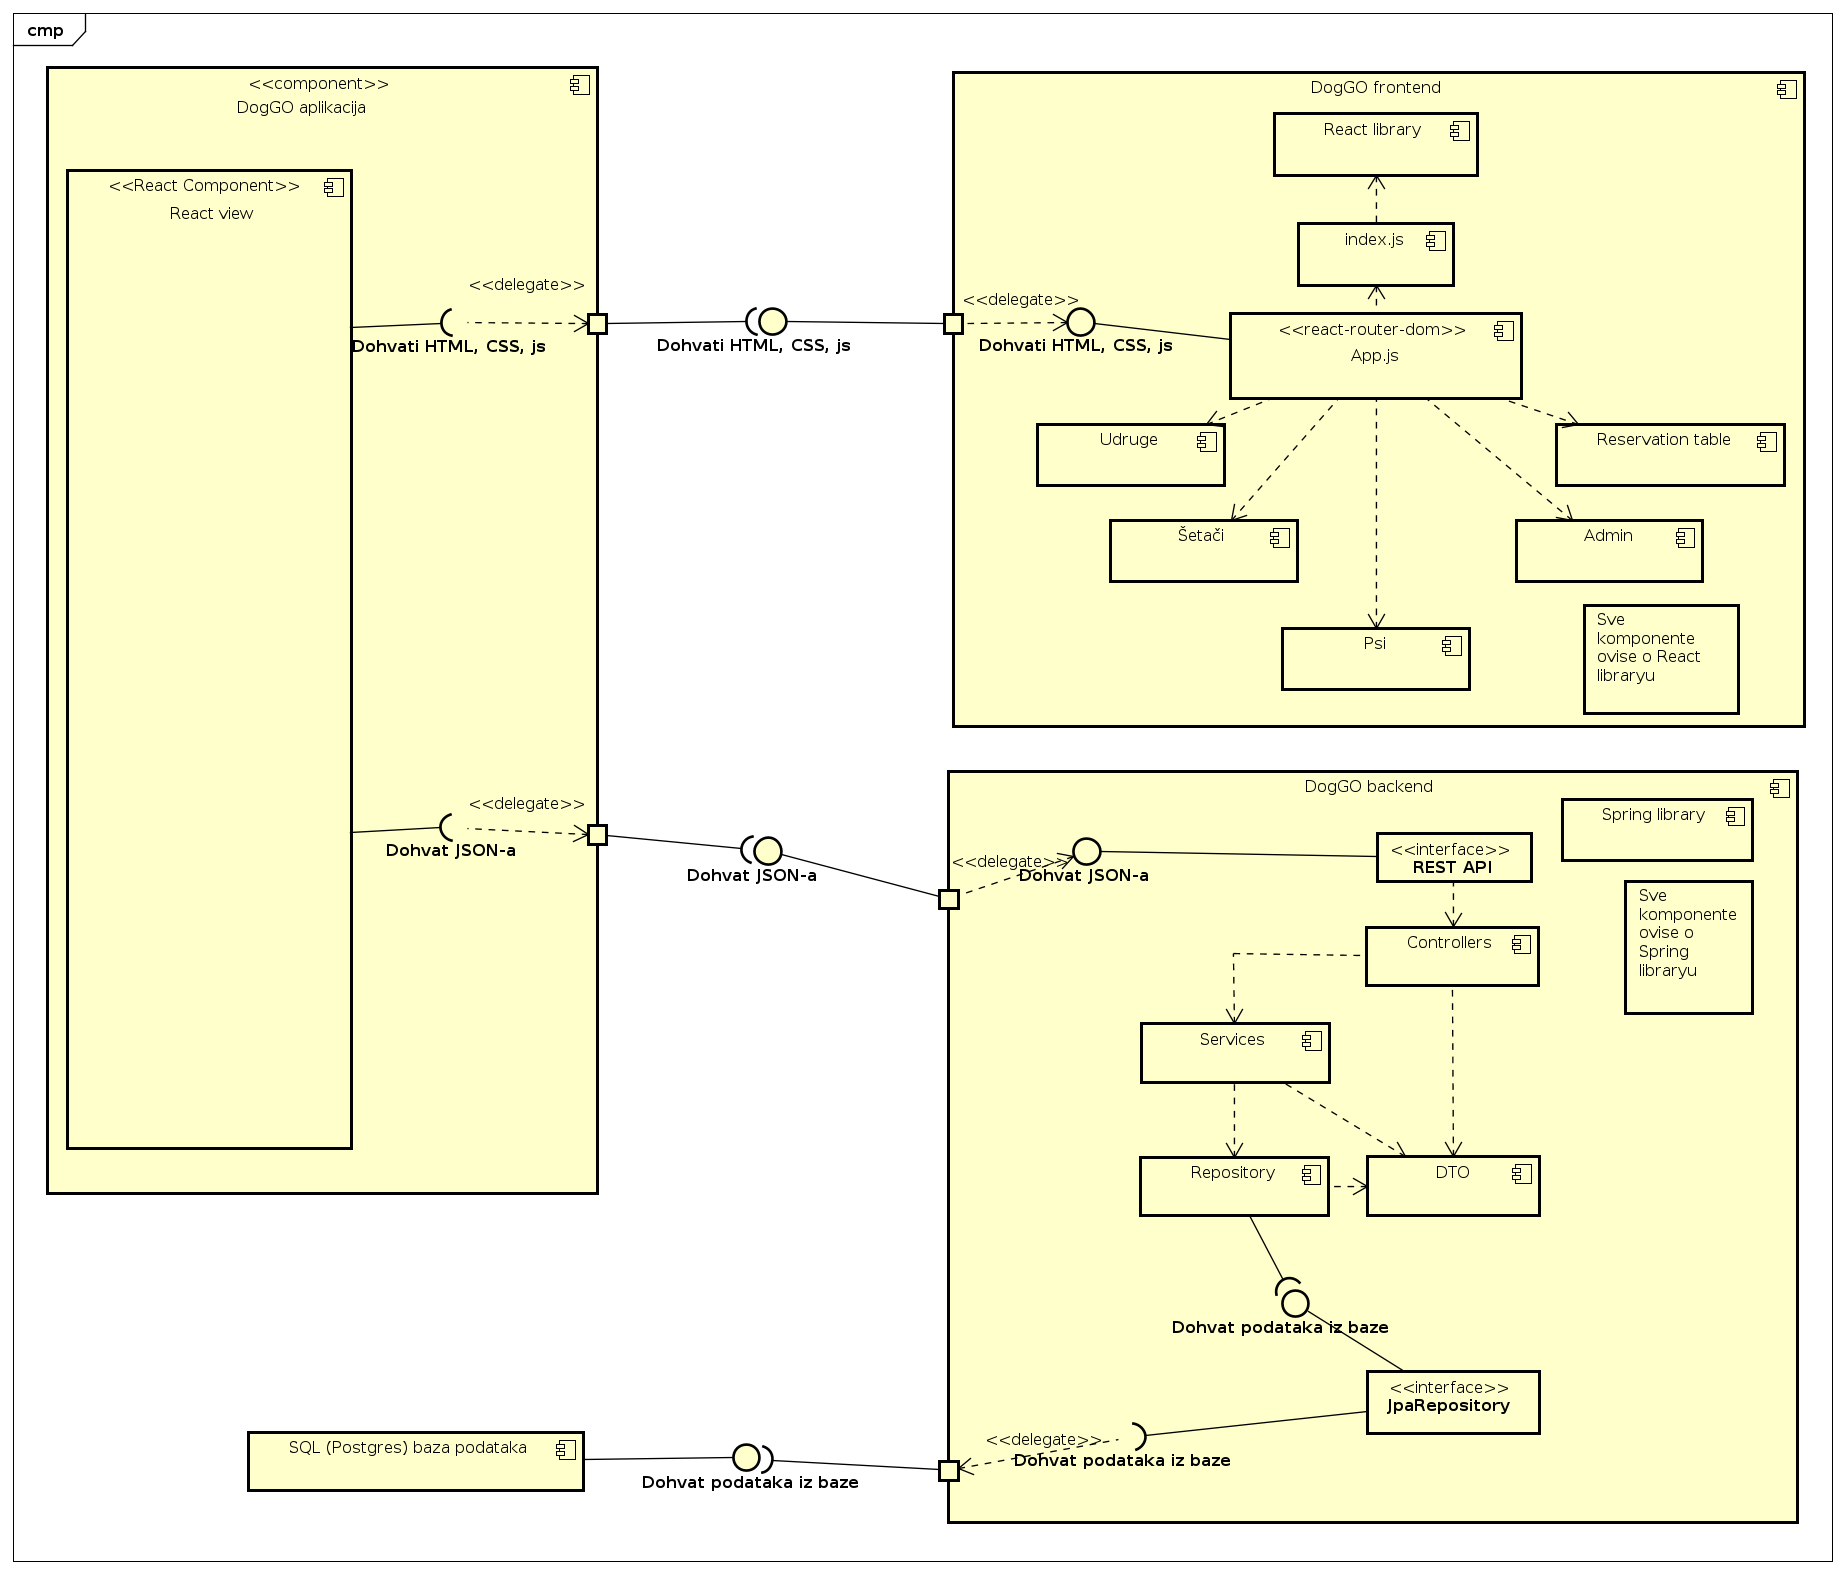
\includegraphics[scale=0.3]{dijagrami/component_diagram.png}
			\centering
			\caption{Dijagram komponenti}
			\label{fig:domain}
		\end{figure}
		